\documentclass[11pt]{article}

%Package
\usepackage[utf8]{inputenc}
\usepackage[margin=0.8in]{geometry}
\usepackage{amsmath}
\usepackage{fancyhdr}
\usepackage{graphicx}
\usepackage{placeins}
\usepackage{listings}
\usepackage{color}
\usepackage[table,xcdraw]{xcolor}
\usepackage{ulem} %barrer du texte
\usepackage{cancel}% barrer dans une expression math (\cancel{})
\usepackage{pgf,tikz}
\usepackage{mathrsfs}
\usepackage{multirow}
%\usepackage{gensymb}
\usepackage{caption}
\usepackage{eurosym}% pour le symbole €



\usetikzlibrary{shapes.geometric, arrows}
\definecolor{qqqqff}{rgb}{0.,0.,1.}
%Configuration
\renewcommand*\contentsname{Sommaire}
\graphicspath{ {images/} }
%\renewcommand{\thesection}{\Roman{section}}
%\renewcommand{\thesubsection}{\Alph{subsection}}

\definecolor{codegreen}{rgb}{0,0.6,0}
\definecolor{codegray}{rgb}{0.5,0.5,0.5}
\definecolor{codepurple}{rgb}{0.58,0,0.82}
\definecolor{backcolour}{rgb}{0.95,0.95,0.92}
 
\lstdefinestyle{mystyle}{
	backgroundcolor=\color{backcolour},   
	commentstyle=\color{codegreen},
	keywordstyle=\color{magenta},
	numberstyle=\tiny\color{codegray},
	stringstyle=\color{codepurple},
	basicstyle=\footnotesize,
	breakatwhitespace=false,         
	breaklines=true,                 
	captionpos=b,                    
	keepspaces=true,                 
	numbers=left,                    
	numbersep=5pt,                  
	showspaces=false,                
	showstringspaces=false,
	showtabs=false,                  
	tabsize=2
}

\lstset{style=mystyle}
\renewcommand{\lstlistingname}{Script}

\title{Rapport TX \\ Banc d'essai : Brushless \& Asynchrone}
\author{Geoffrey Gaillard}
\date{Juin 2016}

\pagestyle{fancy}
\fancyhf{}
\rhead{Geoffrey Gaillard}
\lhead{Banc d'essai : Brushless \& Asynchrone}
\rfoot{Page \thepage}

\begin{document}

\maketitle
\thispagestyle{empty}

\begin{figure}[!h]
    \centering
    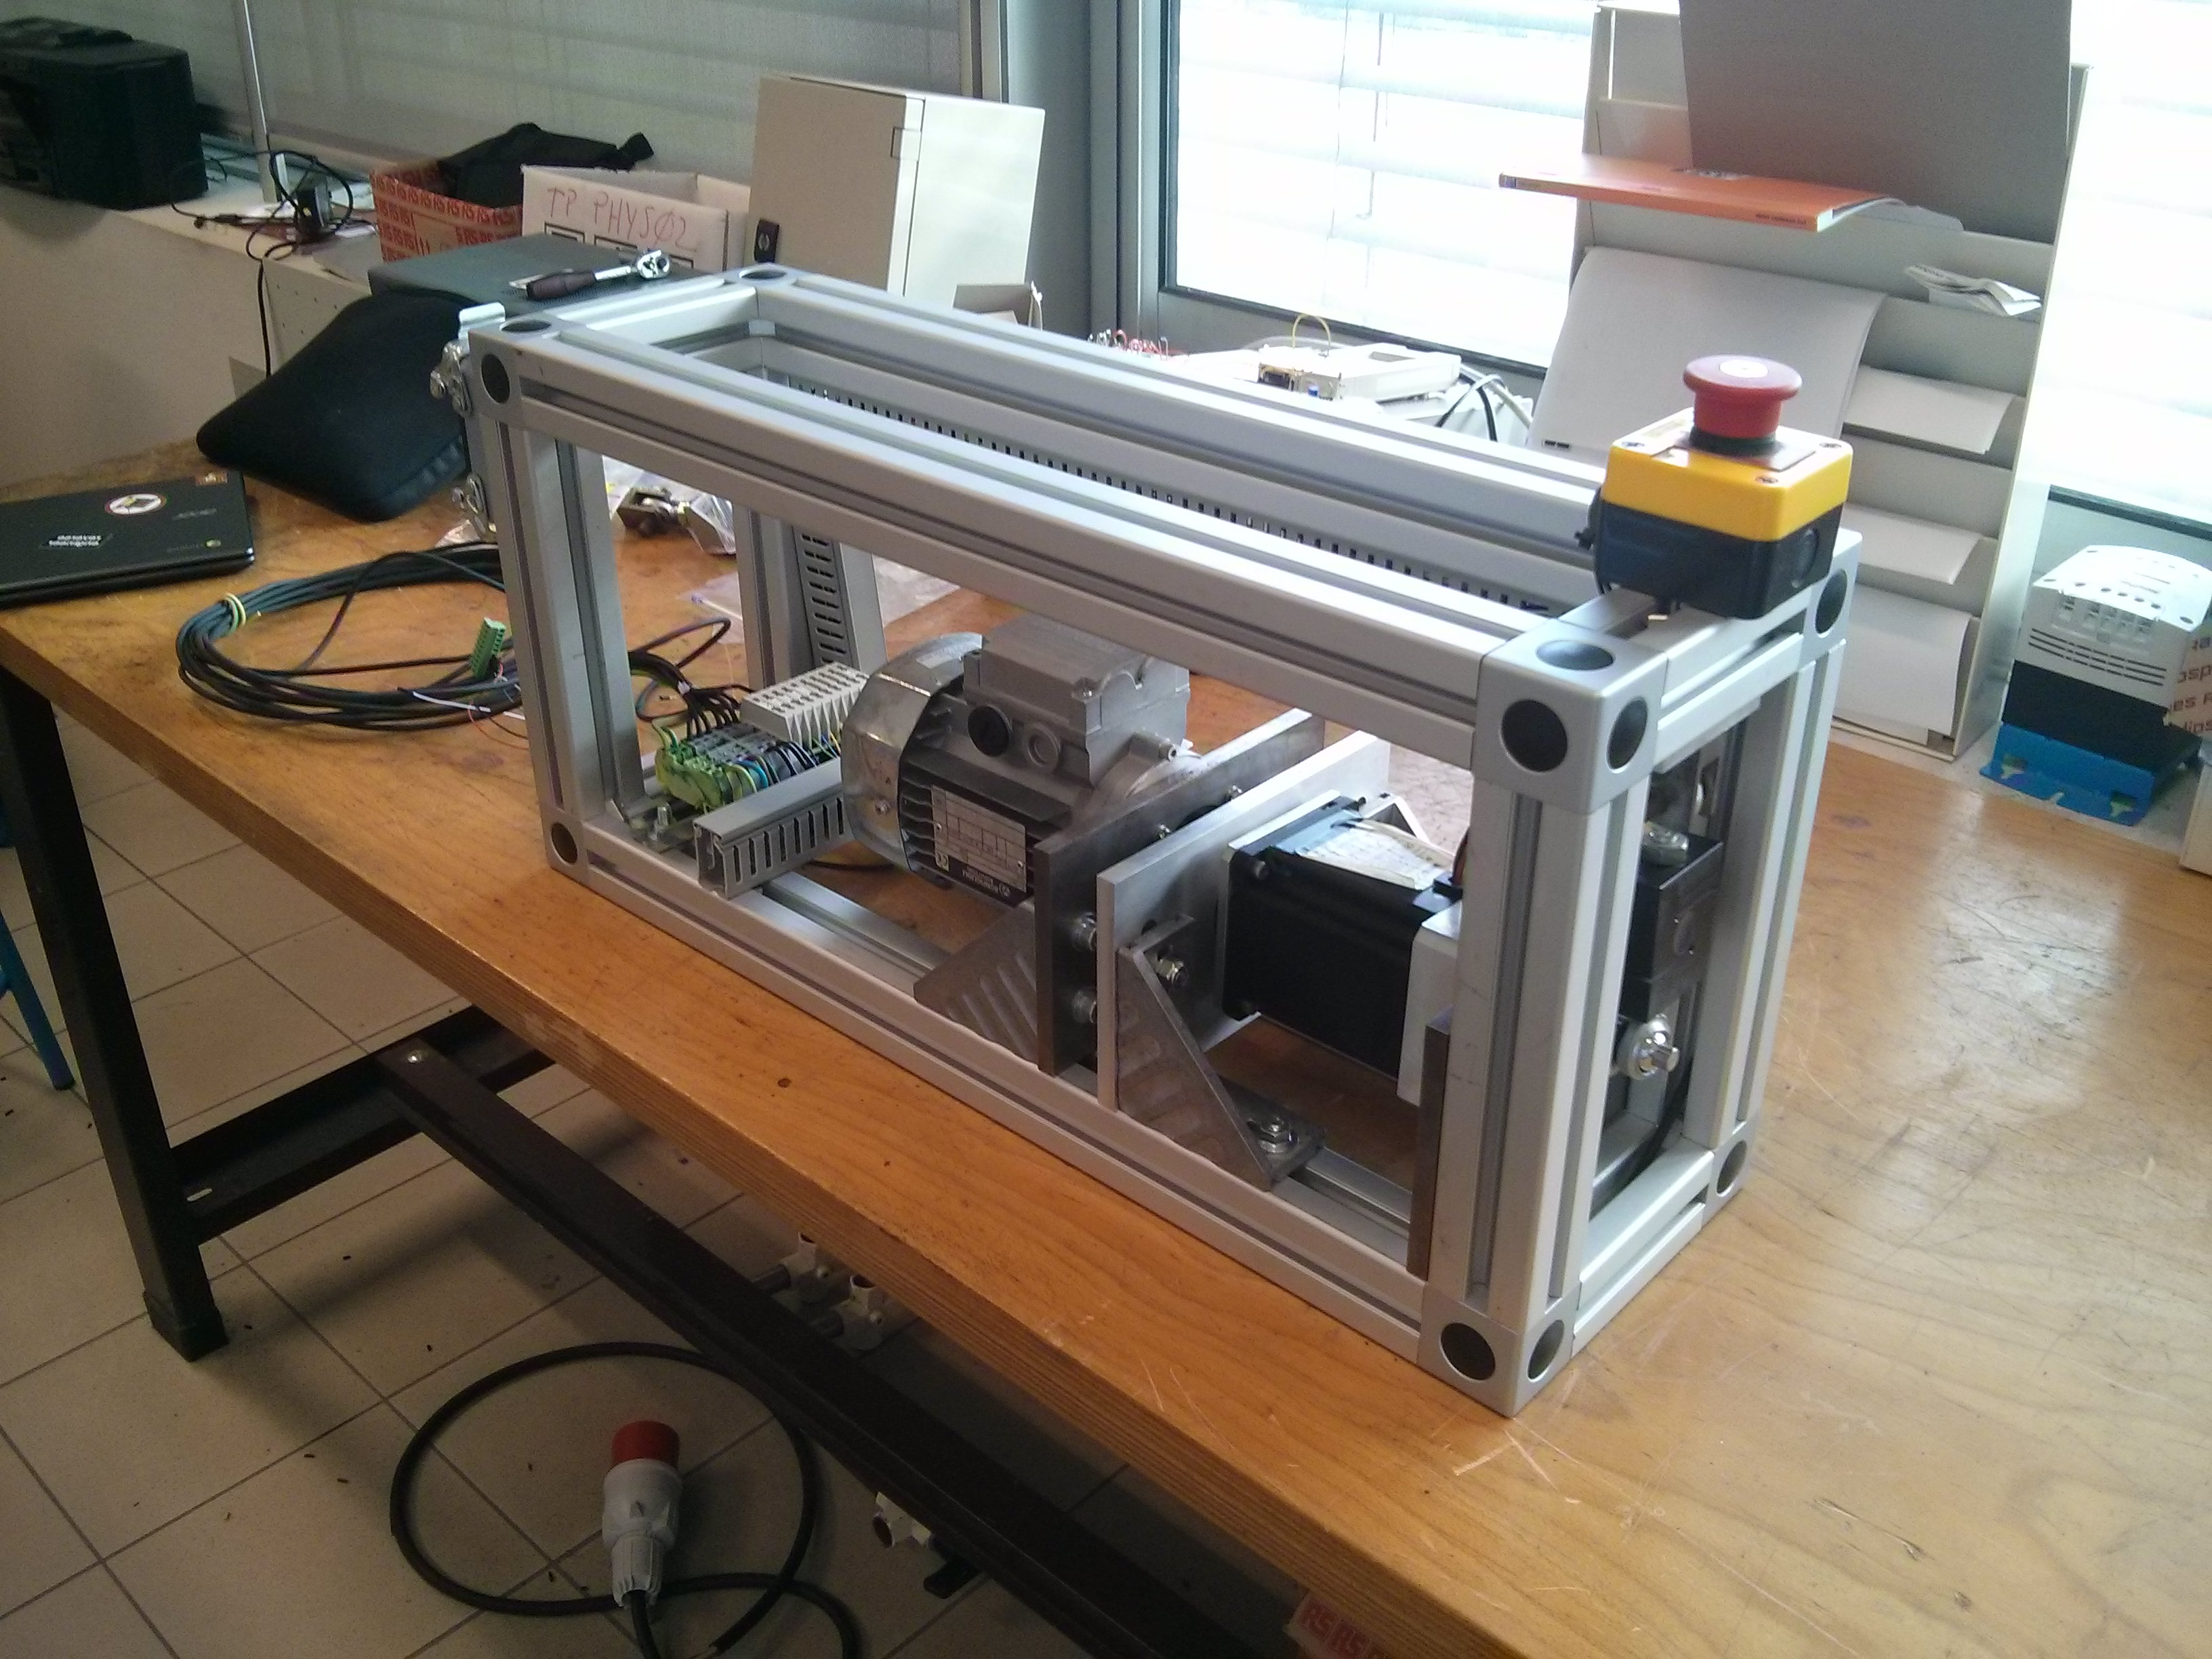
\includegraphics[width=450px]{IMG_20160628_183017.jpg}
    %\caption{figure}
\end{figure}
\newpage

\thispagestyle{empty}
\tableofcontents{}
\newpage

\setcounter{page}{1}
%%%%%%%%%%%%%%%%%%%%%%%%%%%%%%%%%%%%%%%%%%%%%%%%%%%%%%%%%%%%%%%

\section*{Remerciement}

Je vais tous d'abord remercie M. Weil pour l'aide qu'il m'a apporté dans la réalisation de la partie mécanique du banc d'essai, il m'a permit de finaliser le montage de la partie mécanique de façon rapide.\\
M. Didon, pour son aide lors de la réalisation de l'électronique et m'as permis d'améliorer mes compétences en électronique.\\
Ensuite M. Adragna mon encadrant de TX pour m'avoir suivi tous au long de ce projet.\\
Enfin M. Noailles pour l'aide apporter pour la réalisation de ce projet.

\newpage
%%%%%%%%%%%%%%%%%%%%%%%%%%%%%%%%%%%%%%%%%%%%%%%%%%%%%%%%%%%%%%%

\section*{Préambule}

Le projet a consisté à la réalisation d'un banc d'essai composé d'un moteur Brushless et d'un moteur asynchrone dans le but de réaliser des asservissements suivant différentes variables telle que la vitesse d'un des moteurs ou le couple d'un des moteurs. Ce projet a déjà fait l'objet de plusieurs TX sur différents points. La réalisation du pilotage du moteurs asynchrone, la réalisation du pilotage du moteurs Brushless et enfin le banc en lui-même. Lorsque que j'ai pris ce projet, la mécanique était presque complète et une partie de l’électronique avait été réalisé, il me restait donc à rassembler les différents résultats des TX précédentes pour pouvoir finaliser le banc d'essai dans son ensemble. Cependant la partie électrique du banc devait être réalisée à 100\%. Il reste donc beaucoup de travail avant que le banc soit opérationel.

\newpage
%%%%%%%%%%%%%%%%%%%%%%%%%%%%%%%%%%%%%%%%%%%%%%%%%%%%%%%%%%%%%%%

\section{Description du banc d'essai}
Le banc d'essai est composé de 3 éléments :

\begin{itemize}
	\item Le banc d'essai
	\item L'armoire électrique
	\item Le pupitre de commande
\end{itemize}

\subsection{Le banc d'essai}

Le banc d'essai est composé d'un moteur asynchrone et d'un moteur Brushless. Ils sont disposés de telle sorte qu'il sont en vis-à-vis. Ils sont mécaniquement liées par le biais du châssis mais aussi par un accouplement rigide. Ce montage permette de piloter l'un des 2 moteurs, et l'autre joue le rôle de perturbateur ou de simulateur d'inertie.

\paragraph{Mesure \\}

La mesure de vitesse est faite grâce au capteur à effet hall du moteur de Brushless.
\\
La mesure de couple est fait par l'intermédiaire d'un capteur de force placé avec un bras de levier.\\

\begin{figure}[!h]
    \centering
    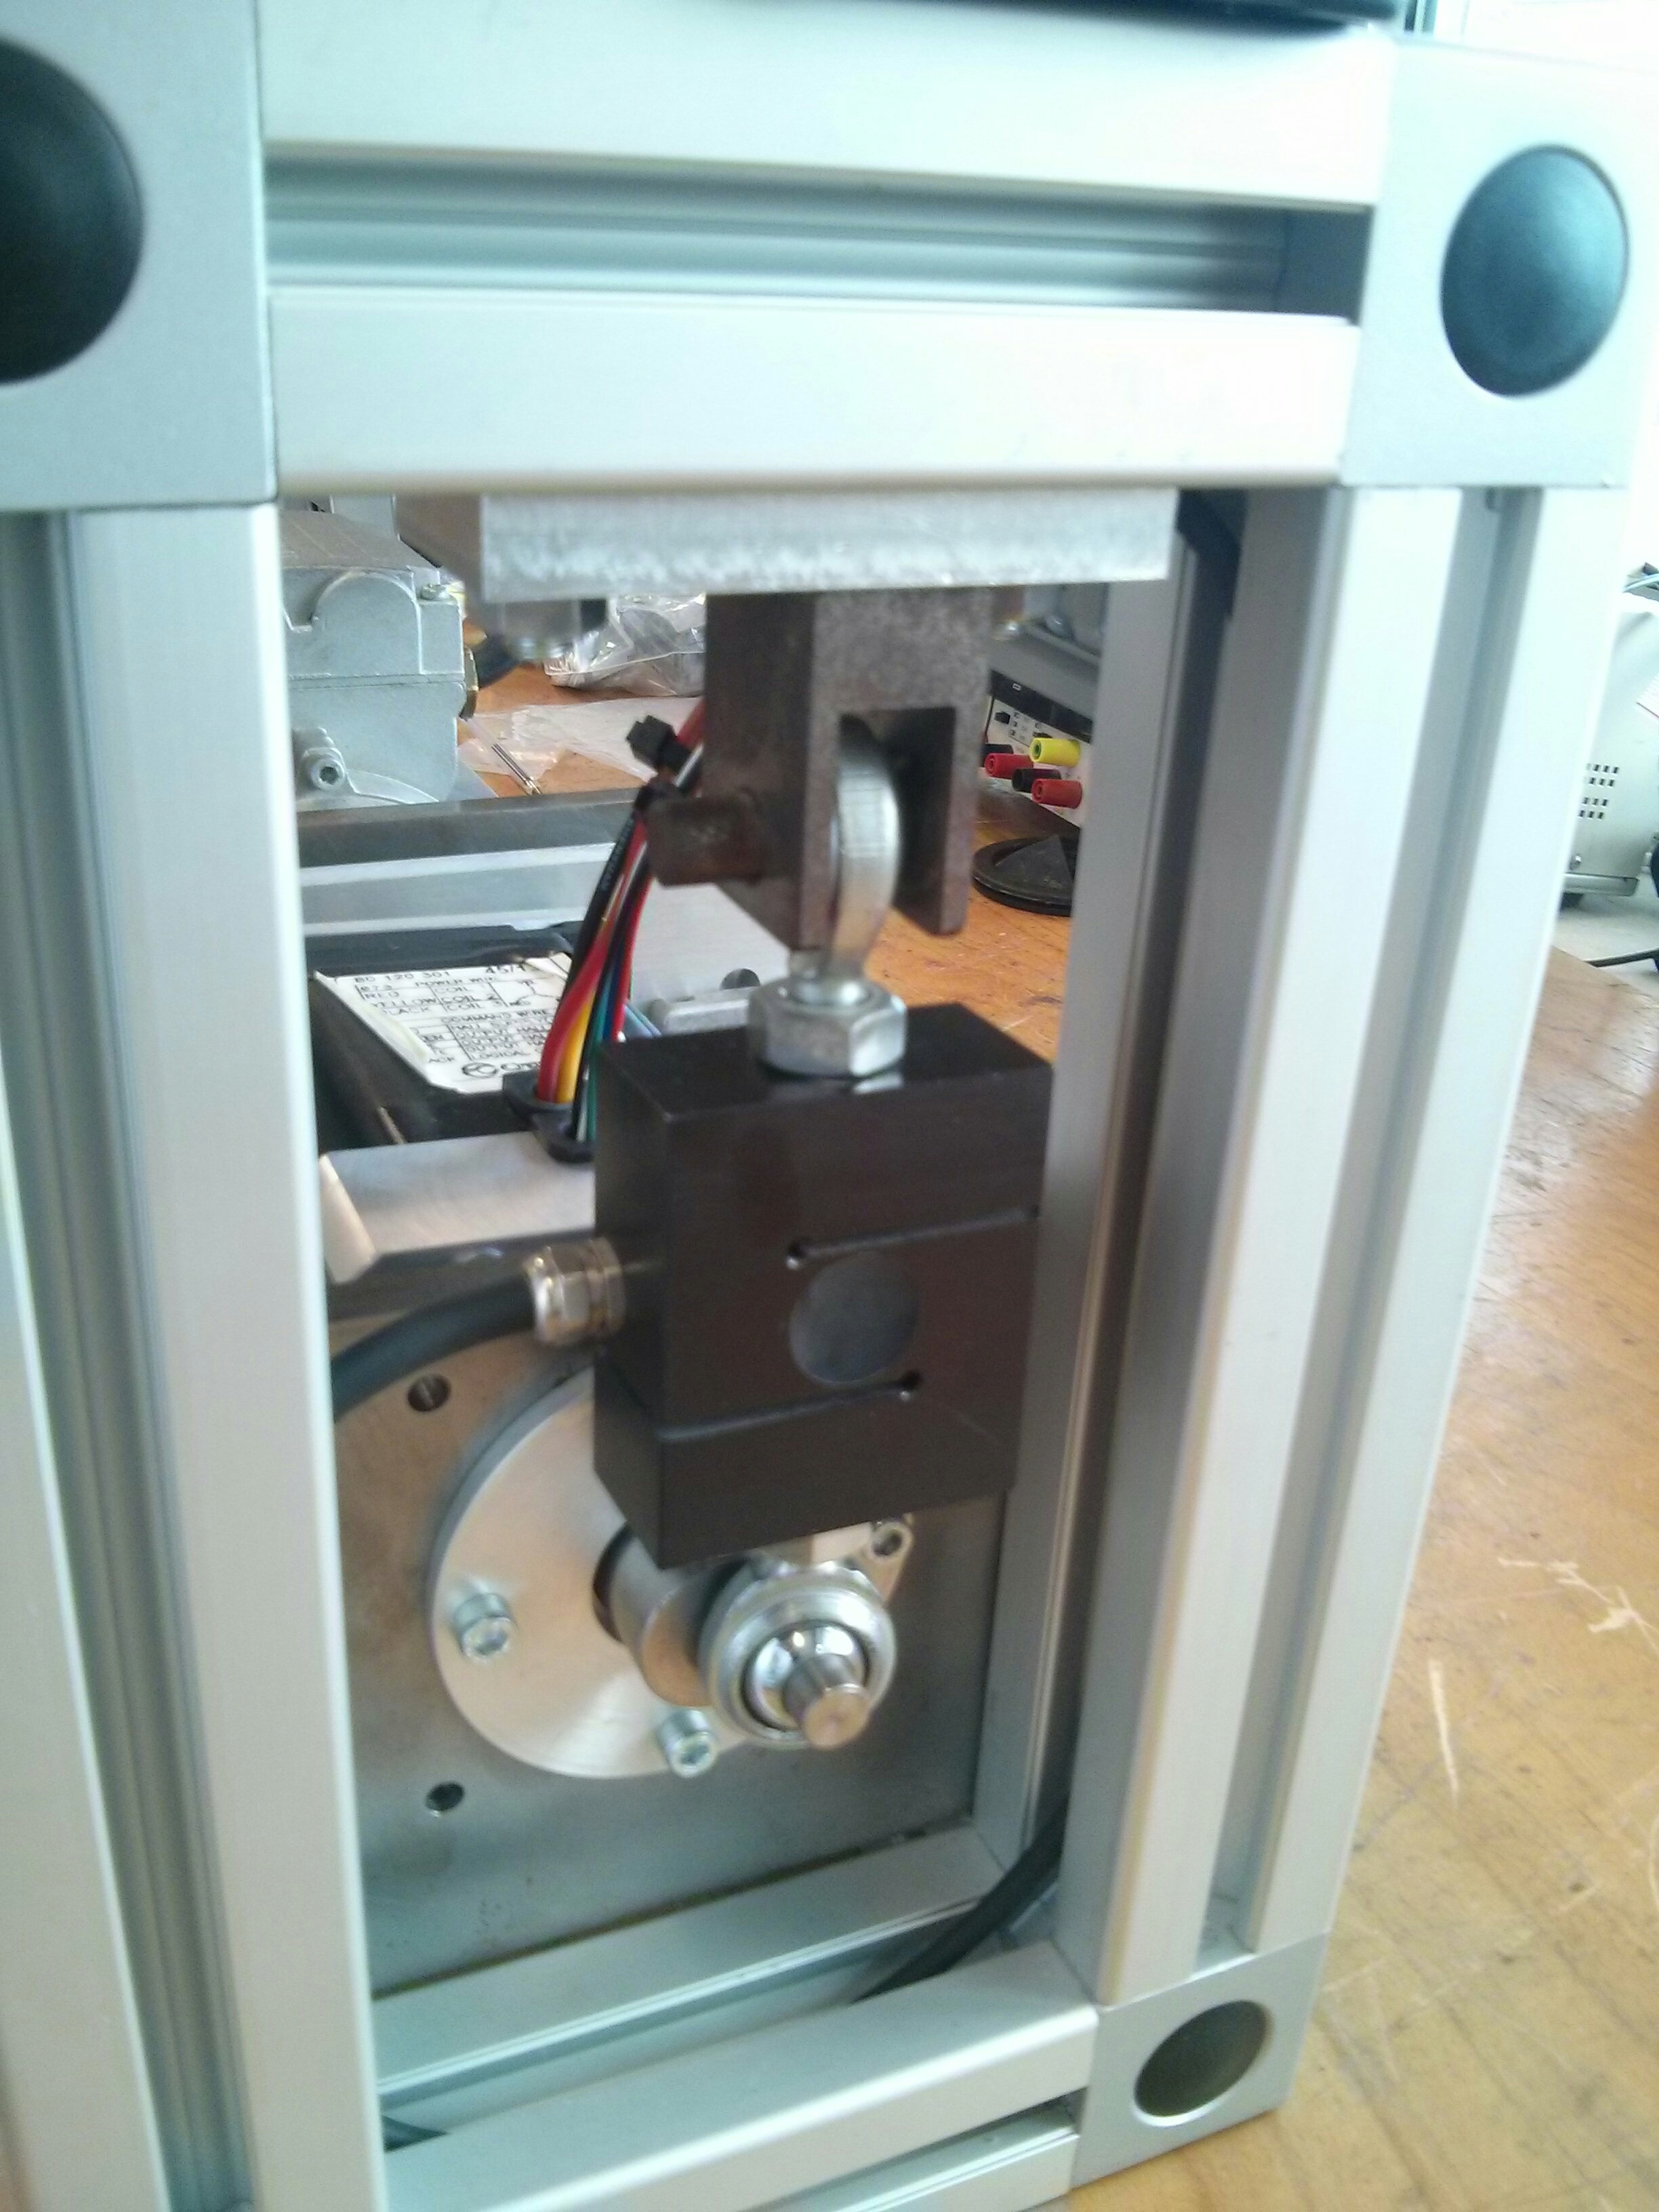
\includegraphics[width=150px]{IMG_20160628_183033.jpg}
    \caption{Capteur de force FN3060}
\end{figure}
\newpage

Le capteur mesure une force de +/- 500 N, le bras de levier est fait de telle sorte que lorsque un moteur est à pleine puissance le capteur de force est presque à sa limite. Ce qui permet de mesurer la puissance mécanique développé par un moteur, dans les 2 sens de rotation. Nous verrons plus tard le traitement des données du capteur.

\subsection{L'armoire électrique}

Celle-ci n'était pas encore réalisé. Pour la faire je me suis inspirer des armoires qui déjà réaliser pour d'autre banc d'essai. Celle-ci était composé d'un seul variateur pour un moteur asynchrones mais toutes la chaine de sécurité et de puissance pouvait être adapté pour le projet. Nous allons voire plus tard les ajout et modification.

\subsection{Le pupitre de commande}
Le pupitre intègre toutes l'électronique de commande, l'ensemble est piloté par une arduino. Il possède aussi une façade avec des potentiomètre, des voyant et des boutons. Pour l'instant le choix du nombre de bouton, potentiomètre et voyant reste indéfinie.


%%%%%%%%%%%%%%%%%%%%%%%%%%%%%%%%%%%%%%%%%%%%%%%%%%%%%%%%%%%%%%%

\section{Électronique}

L'arduino commande l'ensemble des fonctions du banc d'essai, qui sont le contrôle des 2 moteurs. La commande des moteurs ce fait par l'intermédiaire du variateur pour le moteurs asynchrones et par la carte de commande du moteurs Brushless. 

\subsection{Commande asynchrones}

\paragraph{Commande de vitesse \\}
Le moteur asynchrones est piloté en vitesse par une commande 0-10V analogique. L'arduino possède des sorties digital et pour certaine de ces sortie un PWM 0-5V peut-être générer. Il me faut donc transformer le PWM 0-5V en 0-10V analogique. Suite à une petit recherche sur internet j'ai trouvé plusieurs exemple pour réaliser la transformation.\\
\\
\begin{figure}[!h]
    \centering
    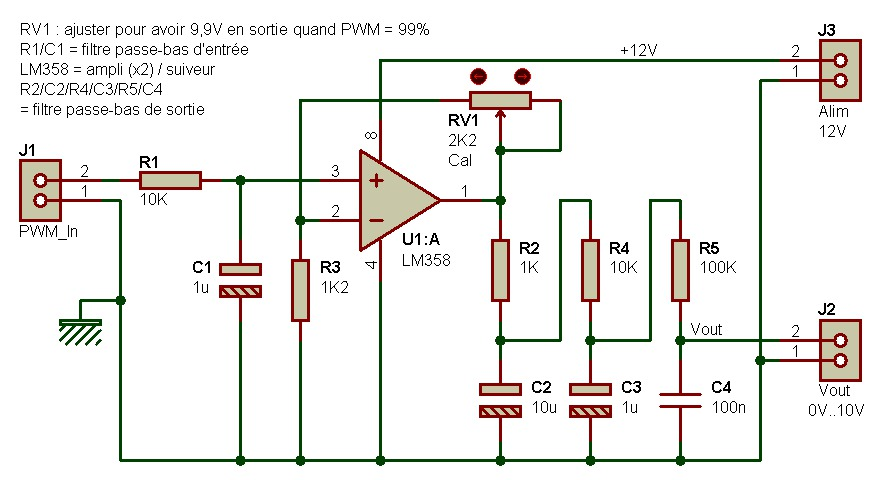
\includegraphics[width=350px]{electronique_conv_pwm_tension.jpg}
    \caption{Schéma de base}
\end{figure}

Le principe du montage est de lissé une première fois le signal par un RC, de l'amplifié et par finir de le lissé par deux RC consécutif. Le système répond instantanément au changement du signal d'entrée.


\begin{figure}[!h]
    \centering
    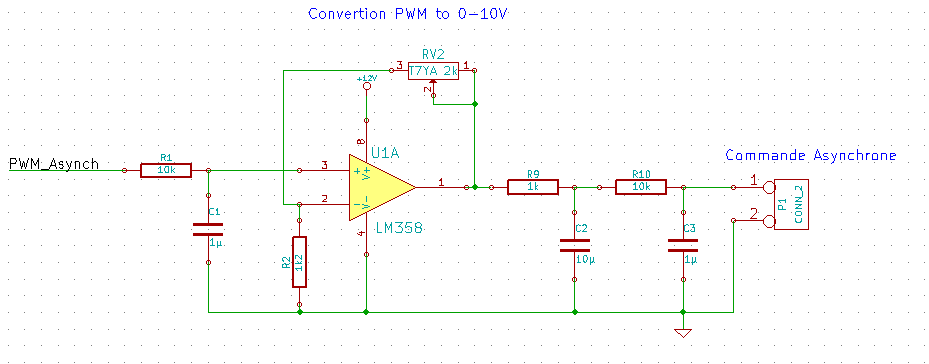
\includegraphics[width=500px]{schema_digt_anolog.png}
    \caption{Schéma de câblage finale}
\end{figure}

\begin{figure}[!h]
    \centering
    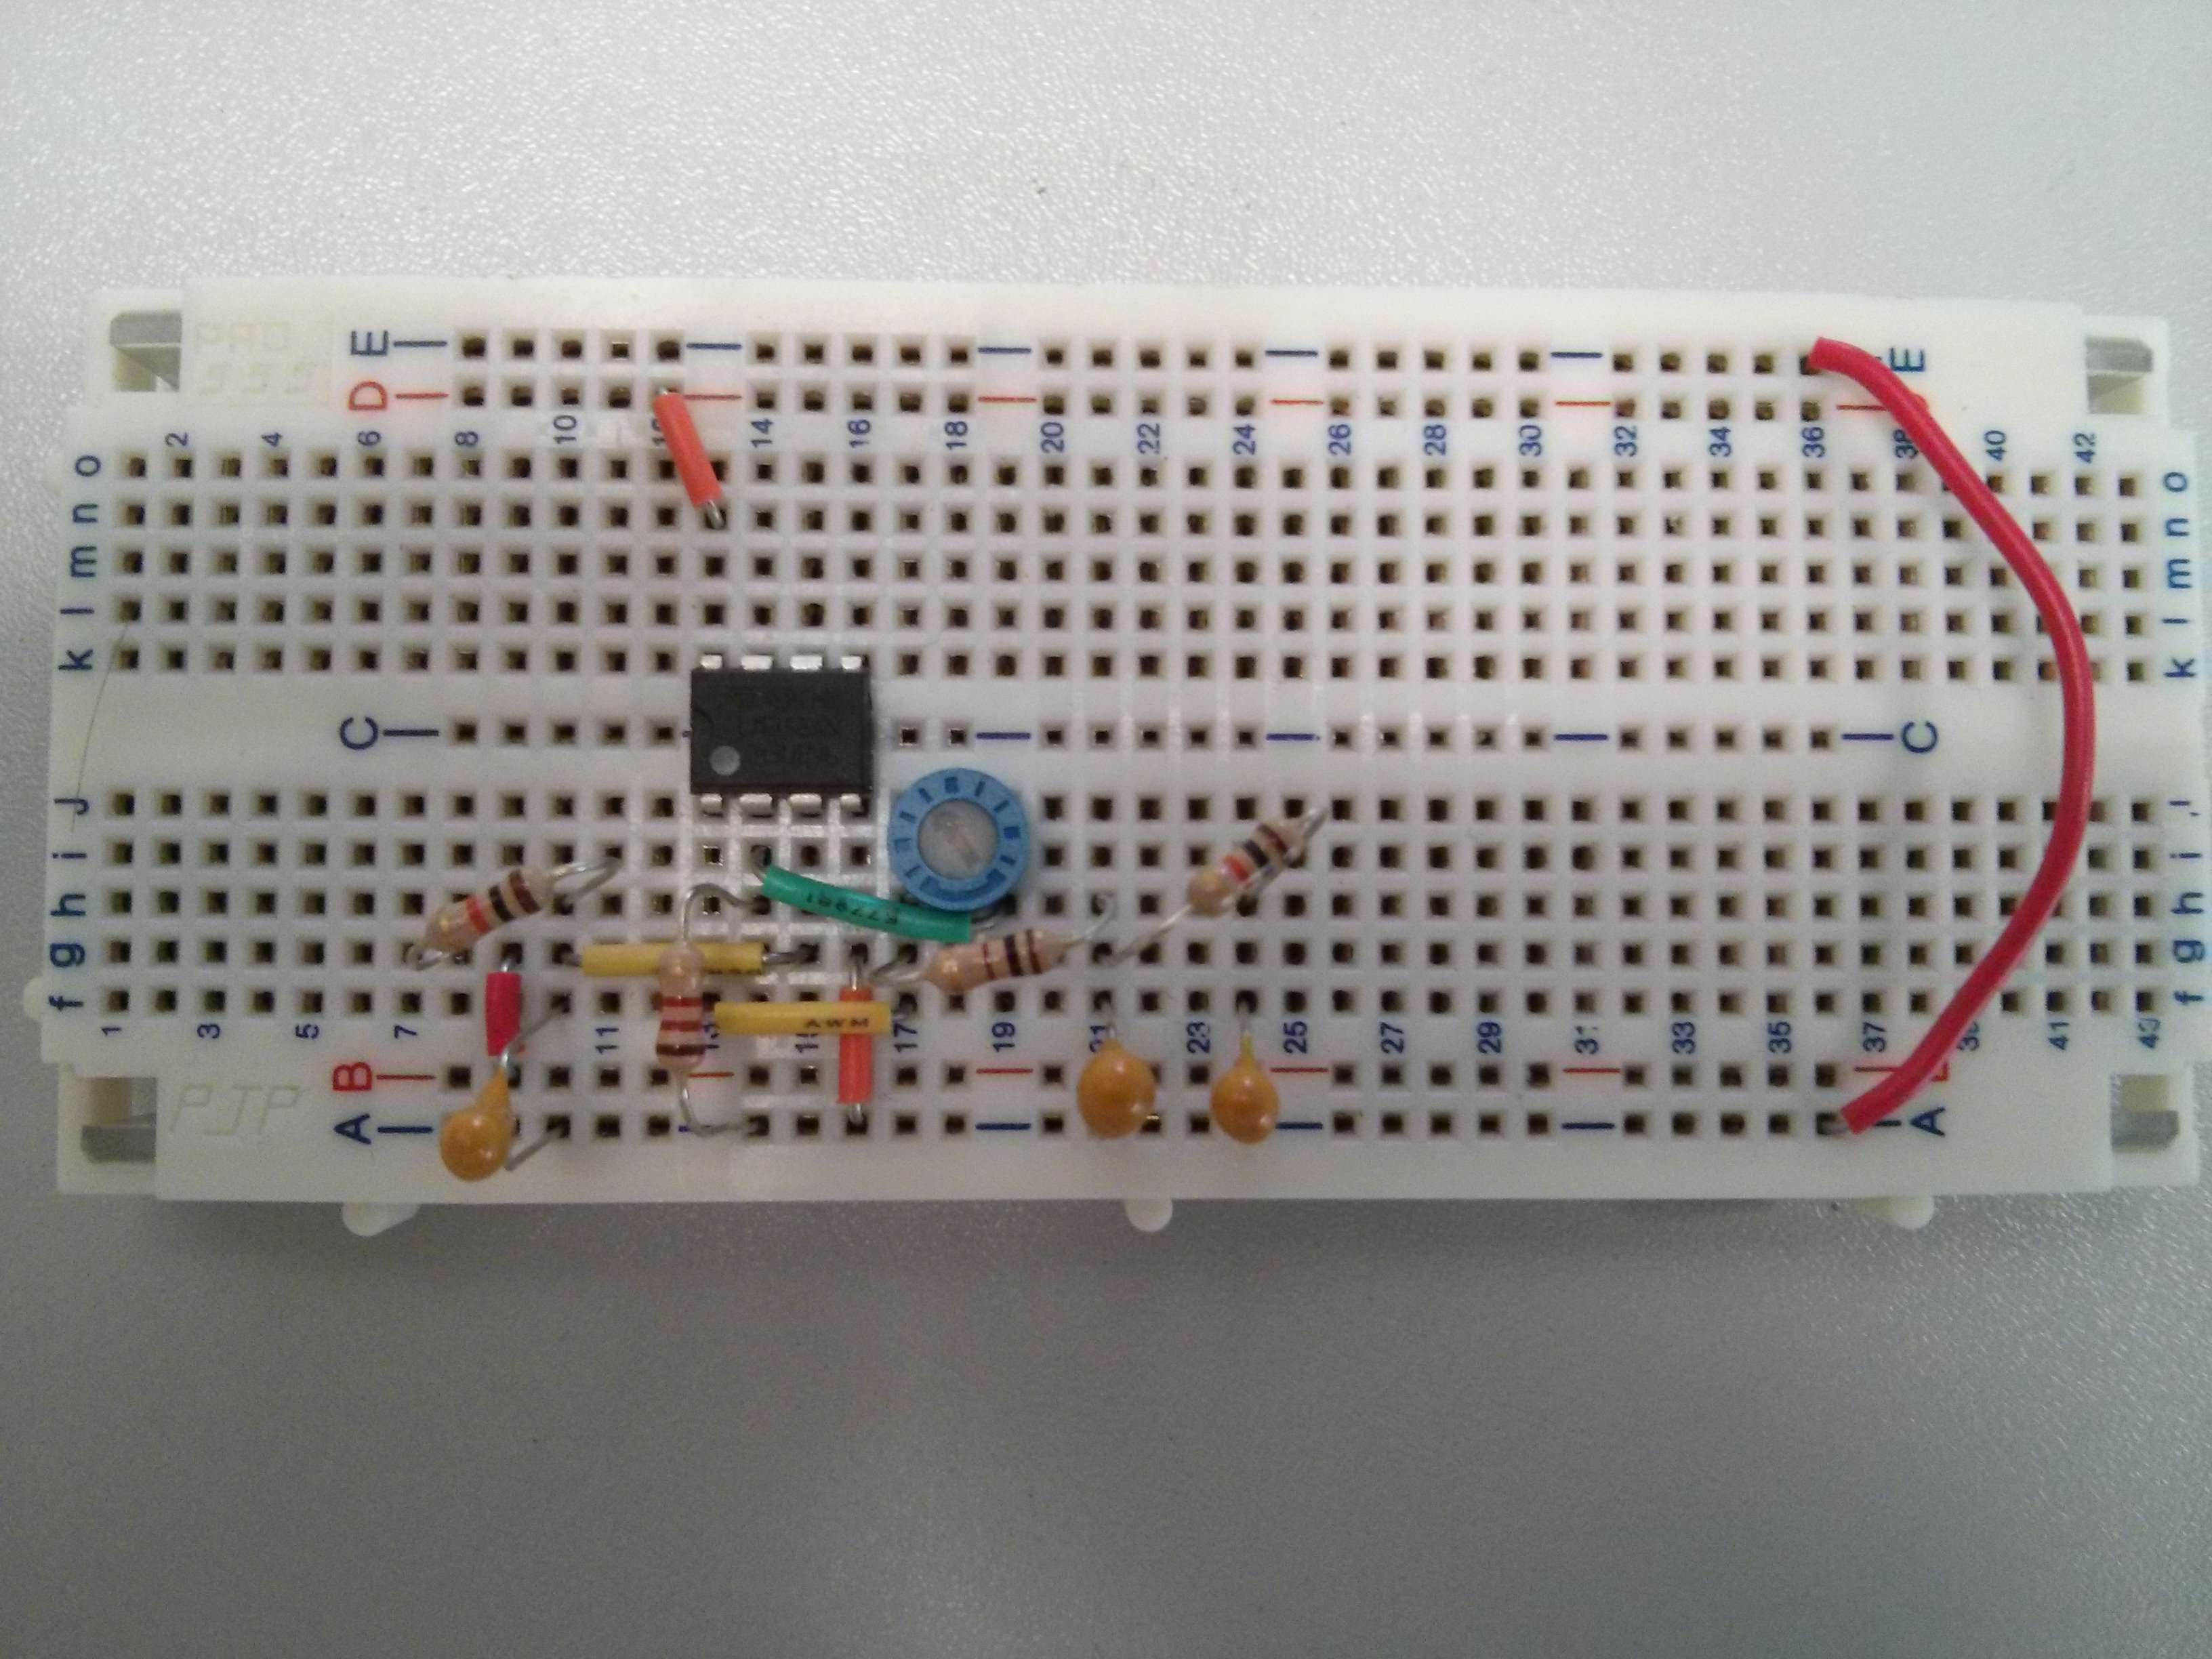
\includegraphics[width=150px]{IMG_20160629_203955.jpg}
    \caption{Montage sur breadboard}
\end{figure}

\paragraph{Commande de marche/arrêt \& sens\\}

Les entrées de marche/arrêt et de sens requière un signal bas à 0V et un signal haut à 24V. Le variateur génère sont propre 24VDC, il suffit donc de récupérer cette tension puis par le biais de transistor BC547, piloter les entrées du variateur voulut.

\begin{figure}[!h]
    \centering
    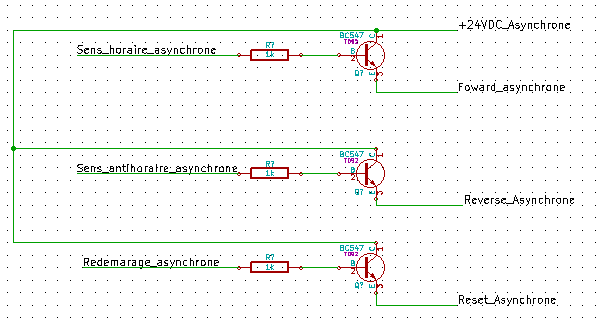
\includegraphics[width=350px]{schema_pilotage_asynchrone.png}
    \caption{Schéma de pilotage asynchrone}
\end{figure}


\subsection{Commande Brushless}

\paragraph{Commande de vitesse \\}

La commande de vitesse pour le contrôleur Brushless peut être du $0-10V$ analogique ou du PWM. La commande se fait par le biais du PWM généré par l'arduino.

\paragraph{Commande Marche/Arrêt \& Sens \\}

Les entrées pour le contrôleur Brushless ont des niveaux logique compatible avec l'arduino. État 0 : $<2V$ ; état 1 : $<4V$. Donc pas besoin d'électronique supplémentaire pour la commande du moteur Brushless\\
\\
La partie commande est donc complète, nous voulons commander les moteurs en boucle fermé il nous faut donc les retours vers l'arduino des signaux de vitesse et de force.

\paragraph{Entrée encoder \& direction}

Pour connaître la vitesse des moteurs je récupère la sortie encoder donnée par le controleurs brushless, de même pour le sens de rotation réel. Cependant un petite adaptation doit être réaliser, les tensions fournit ne corresponde $V_{max} = 28,5V$. Un petit pont diviseur de tension est réaliser.

\begin{figure}[!h]
    \centering
    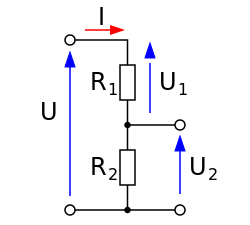
\includegraphics[width=150px]{Pont_diviseur.png}
    \caption{Schéma du pont diviseur de tension}
\end{figure}

\begin{equation}
 	\begin{split}
		U_{2} &= U \frac{R_{2}}{R_{1}+R_{2}}\\
		U &= 28,5 V\\
		U_{2} &= 5V\\
		R_{2} &= 10k\Omega\\
		\Rightarrow R_{1} &= 47k\Omega\\
	\end{split}
\end{equation}


\subsection{Capteur de force}

Pour cette partie je me suis basé sur la TX de Renhai PU.\\
J'utilise un capteur de force FN3060. Le capteur fonctionne avec un pont de wheatstone. \\
\\
Suivant la documentation le capteur doit être alimenté en $10V$ et le signal de sortie est fonction de cette alimentation $2mV/V$. Donc pour une alimentation de $10V$ le signal de sortie est donc compris entre $ [-20mV ; +20mV] $. Pour une force de 500N nous avons donc en sortie une tension de 20mV. Ce qui est extrêmement faible et pas lisible pour une arduino (par défaut la résolution de l'arduino en lecture d'un signal analogique : $\frac{5V}{1024 bit} $). De plus, le signal peut être aussi négatif. Nous ne pouvons nous restreindre à un seul sens de rotation des moteurs pour nous permettre de mesurer un couple c'est pour quoi il faut traiter le signal du capteur.\\
\\
Dans la TX de Renhai PU, il à réalisé sur breadboard un montage pour permettre la lecture du signal par une arduino. J'ai repris ce montage puis testé. Il c'est avéré qu'il y avait quelque erreur de câblage, cependant, je n'ai pas réussi à faire fonctionner le montage complait. J'ai donc repris la démarche qu'il avait entrepris mais en essayant de dissocier un maximum les étapes.\\
\\
Le but du montage est de récupéré un signal lisible par l'arduino : Signal positif entre 0-5V. Mon signal d'entrée peut être négatif et positif, je doit donc passé la partie négative en positive. Cependant comparé à Renhai PU, la lecture du signal par l'arduino se fera par 3 entrées : signal positif, signa négatif (mais redresser), sens. Le signal sens est redondant par rapport au 2 autres mais il y a cependant un seuil non nul lorsque le capteur 	est repos.\\
\\
Le signal doit être amplifié 250 fois ($20mV \rightarrow 5V$). Il sera amplifié en plusieurs étapes. 

\paragraph{Amplificateur différentiel}
Ce montage permet la soustraction de signaux. Il permet de changer de référence et de passé au GND commun à toutes l'électronique, les signaux sont donc combiner. On réaliser aussi un première amplification.\\

\begin{figure}[!h]
	\centering
	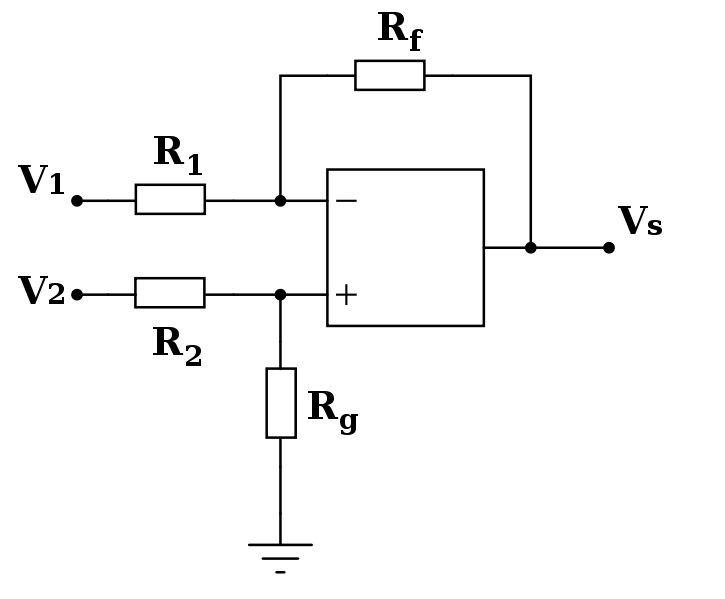
\includegraphics[width=150px]{AOP_dif.png}
	\caption{Montage AOP différentiel}
\end{figure}
\FloatBarrier

Je me place dans le cas : $R_{1} = R_{2}$ \&  $R_{f} = R_{g}$   

\begin{equation}
	V_{s} = \frac{R_{f}}{R_{1}}(V_{2}-V_{1})
\end{equation}

On ce place dans le cas $V_{2}-V_{1} = 20mV$ et on amplifie le signal jusqu'à $2,5V$
		
\begin{equation}
	 \begin{split}
		R_{1} &= 100 \Omega\\
		\frac{R_{f}}{R_{1}} &= 125\\
		\Rightarrow R_{f} &= 125*100\\
		&= 12500 \Omega\\
		\Rightarrow &= 12000 \Omega\\
		\Rightarrow Vs_{max} &= +/-2,4V 
	\end{split}
\end{equation}

\paragraph{Amplificateur inverseur}

Pour récupérer la partie négative du signal on l'inverse puis une diode pour supprimer la partie négative.

\begin{figure}[!h]
	\centering
	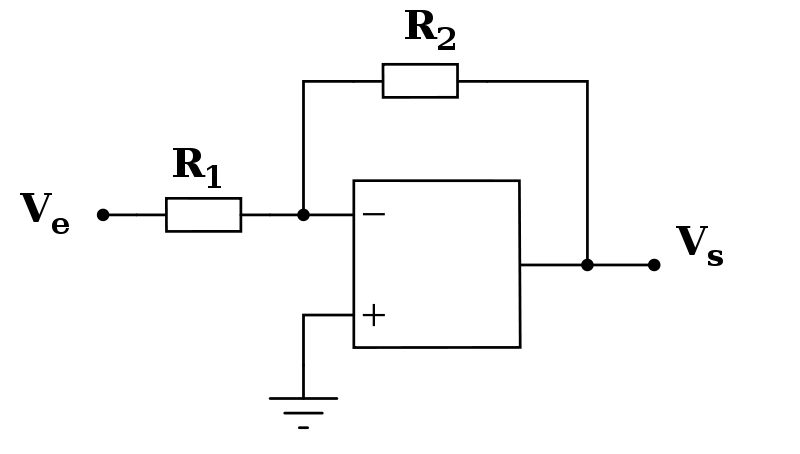
\includegraphics[width=150px]{AOP_inv.png}
	\caption{Montage AOP inverseur}
\end{figure}
\FloatBarrier

Je part du principe du le signal d'entrée maximum $V_{s} = 2,5V$. Je dois donc amplifier le signal 2 fois.

\begin{equation}
	 \begin{split}
		V_{s} &= - V_{e} \frac{R_{2}}{R_{1}}\\
		R_{1} &= 1k\Omega\\
		\frac{R_{2}}{R_{1}} &= 2\\
		\Rightarrow R_{2} &= 2 * R_{1}\\
		&= 2k\Omega
	\end{split}
\end{equation}

Pour permettre le réglage du gain, $R_{2}$ sera composé de 2 résistance en série. Une résistance de $1,5k\Omega$ et un trimer de $1k\Omega$, ce qui permette un réglage de gain sur une grande plage.

\paragraph{Amplificateur non inverseur}

Pour récupérer la partie positive le même principe est appliqué que pour l'amplificateur inverseur.

\begin{figure}[!h]
	\centering
	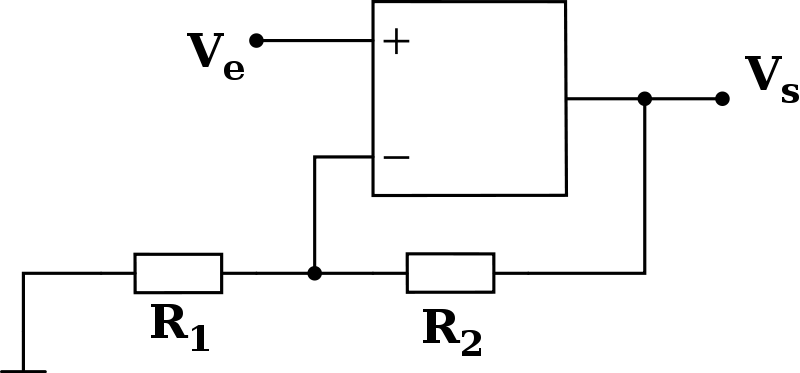
\includegraphics[width=150px]{AOP_amp.png}
	\caption{Montage AOP inverseur}
\end{figure}
\FloatBarrier

Je part du principe du le signal d'entrée maximum $V_{s} = 2,5V$. Je dois donc amplifier le signal 2 fois.

\begin{equation}
	 \begin{split}
		V_{s} &= V_{e} (1+\frac{R_{2}}{R_{1}})\\
		R_{1} &= 1k\Omega\\
		1+\frac{R_{2}}{R_{1}} &= 2\\
		\Rightarrow R_{2} &= 2 R_{1}\\
		&= 2k\Omega
	\end{split}
\end{equation}

Pour permettre le réglage du gain, $R_{2}$ sera composé de 2 résistance en série. Une résistance de $0,5k\Omega$ et un trimer de $1k\Omega$, ce qui permette un réglage de gain sur une grande plage.

\paragraph{Comparateur}

Un montage comparateur permet la détection du sens de la force. 

\begin{figure}[!h]
	\centering
	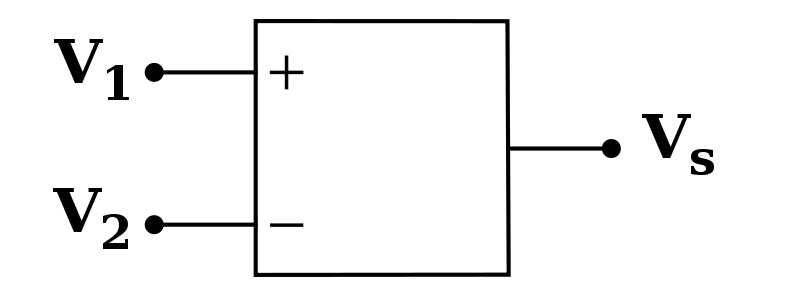
\includegraphics[width=150px]{AOP_comp.png}
	\caption{Montage AOP inverseur}
\end{figure}
\FloatBarrier

\begin{equation}
	V_{s} = 
	\left\{
	  \begin{array}{rcr}
	    V_{s+}& \; V_{1}>V_{2} \\
	    V_{s-}& \; V_{1}<V_{2} \\
	  \end{array}
	\right.
\end{equation}

$V_{1}$ est relié à la masse se qui donne comme résultat :

\begin{equation}
 	\begin{split}
		si \; V_{2} > 0 \\
		\Rightarrow V_{s} < 0 \\			
		si \; V_{2} < 0 \\
		\Rightarrow V_{s} > 0 \\			
	\end{split}
\end{equation}

La détection du sens négatif de la force est fait à l'état haut.

\begin{figure}[!h]
    \centering
    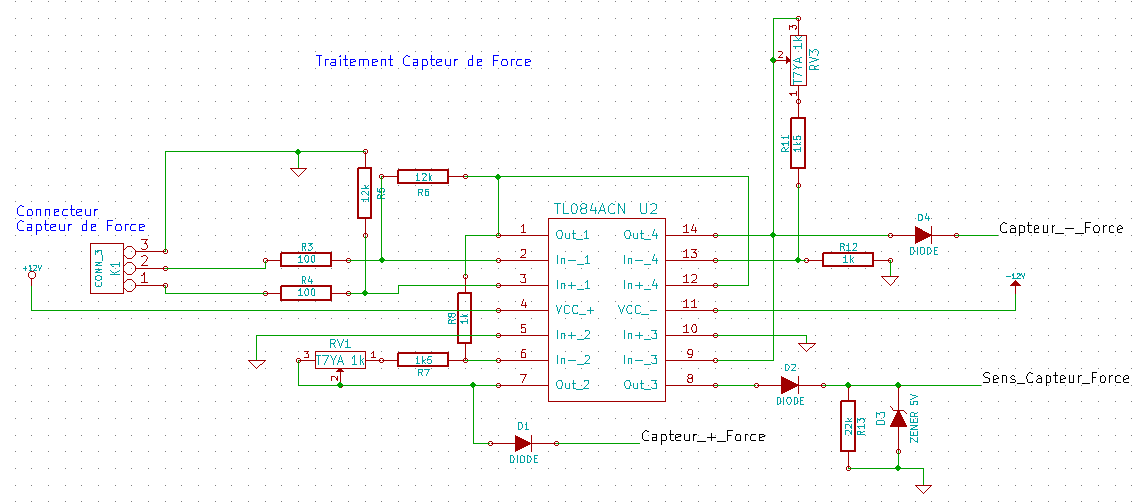
\includegraphics[width=500px]{schema_force.png}
    \caption{Schéma traitement du signal du capteur de force}
\end{figure}

\begin{figure}[!h]
    \centering
    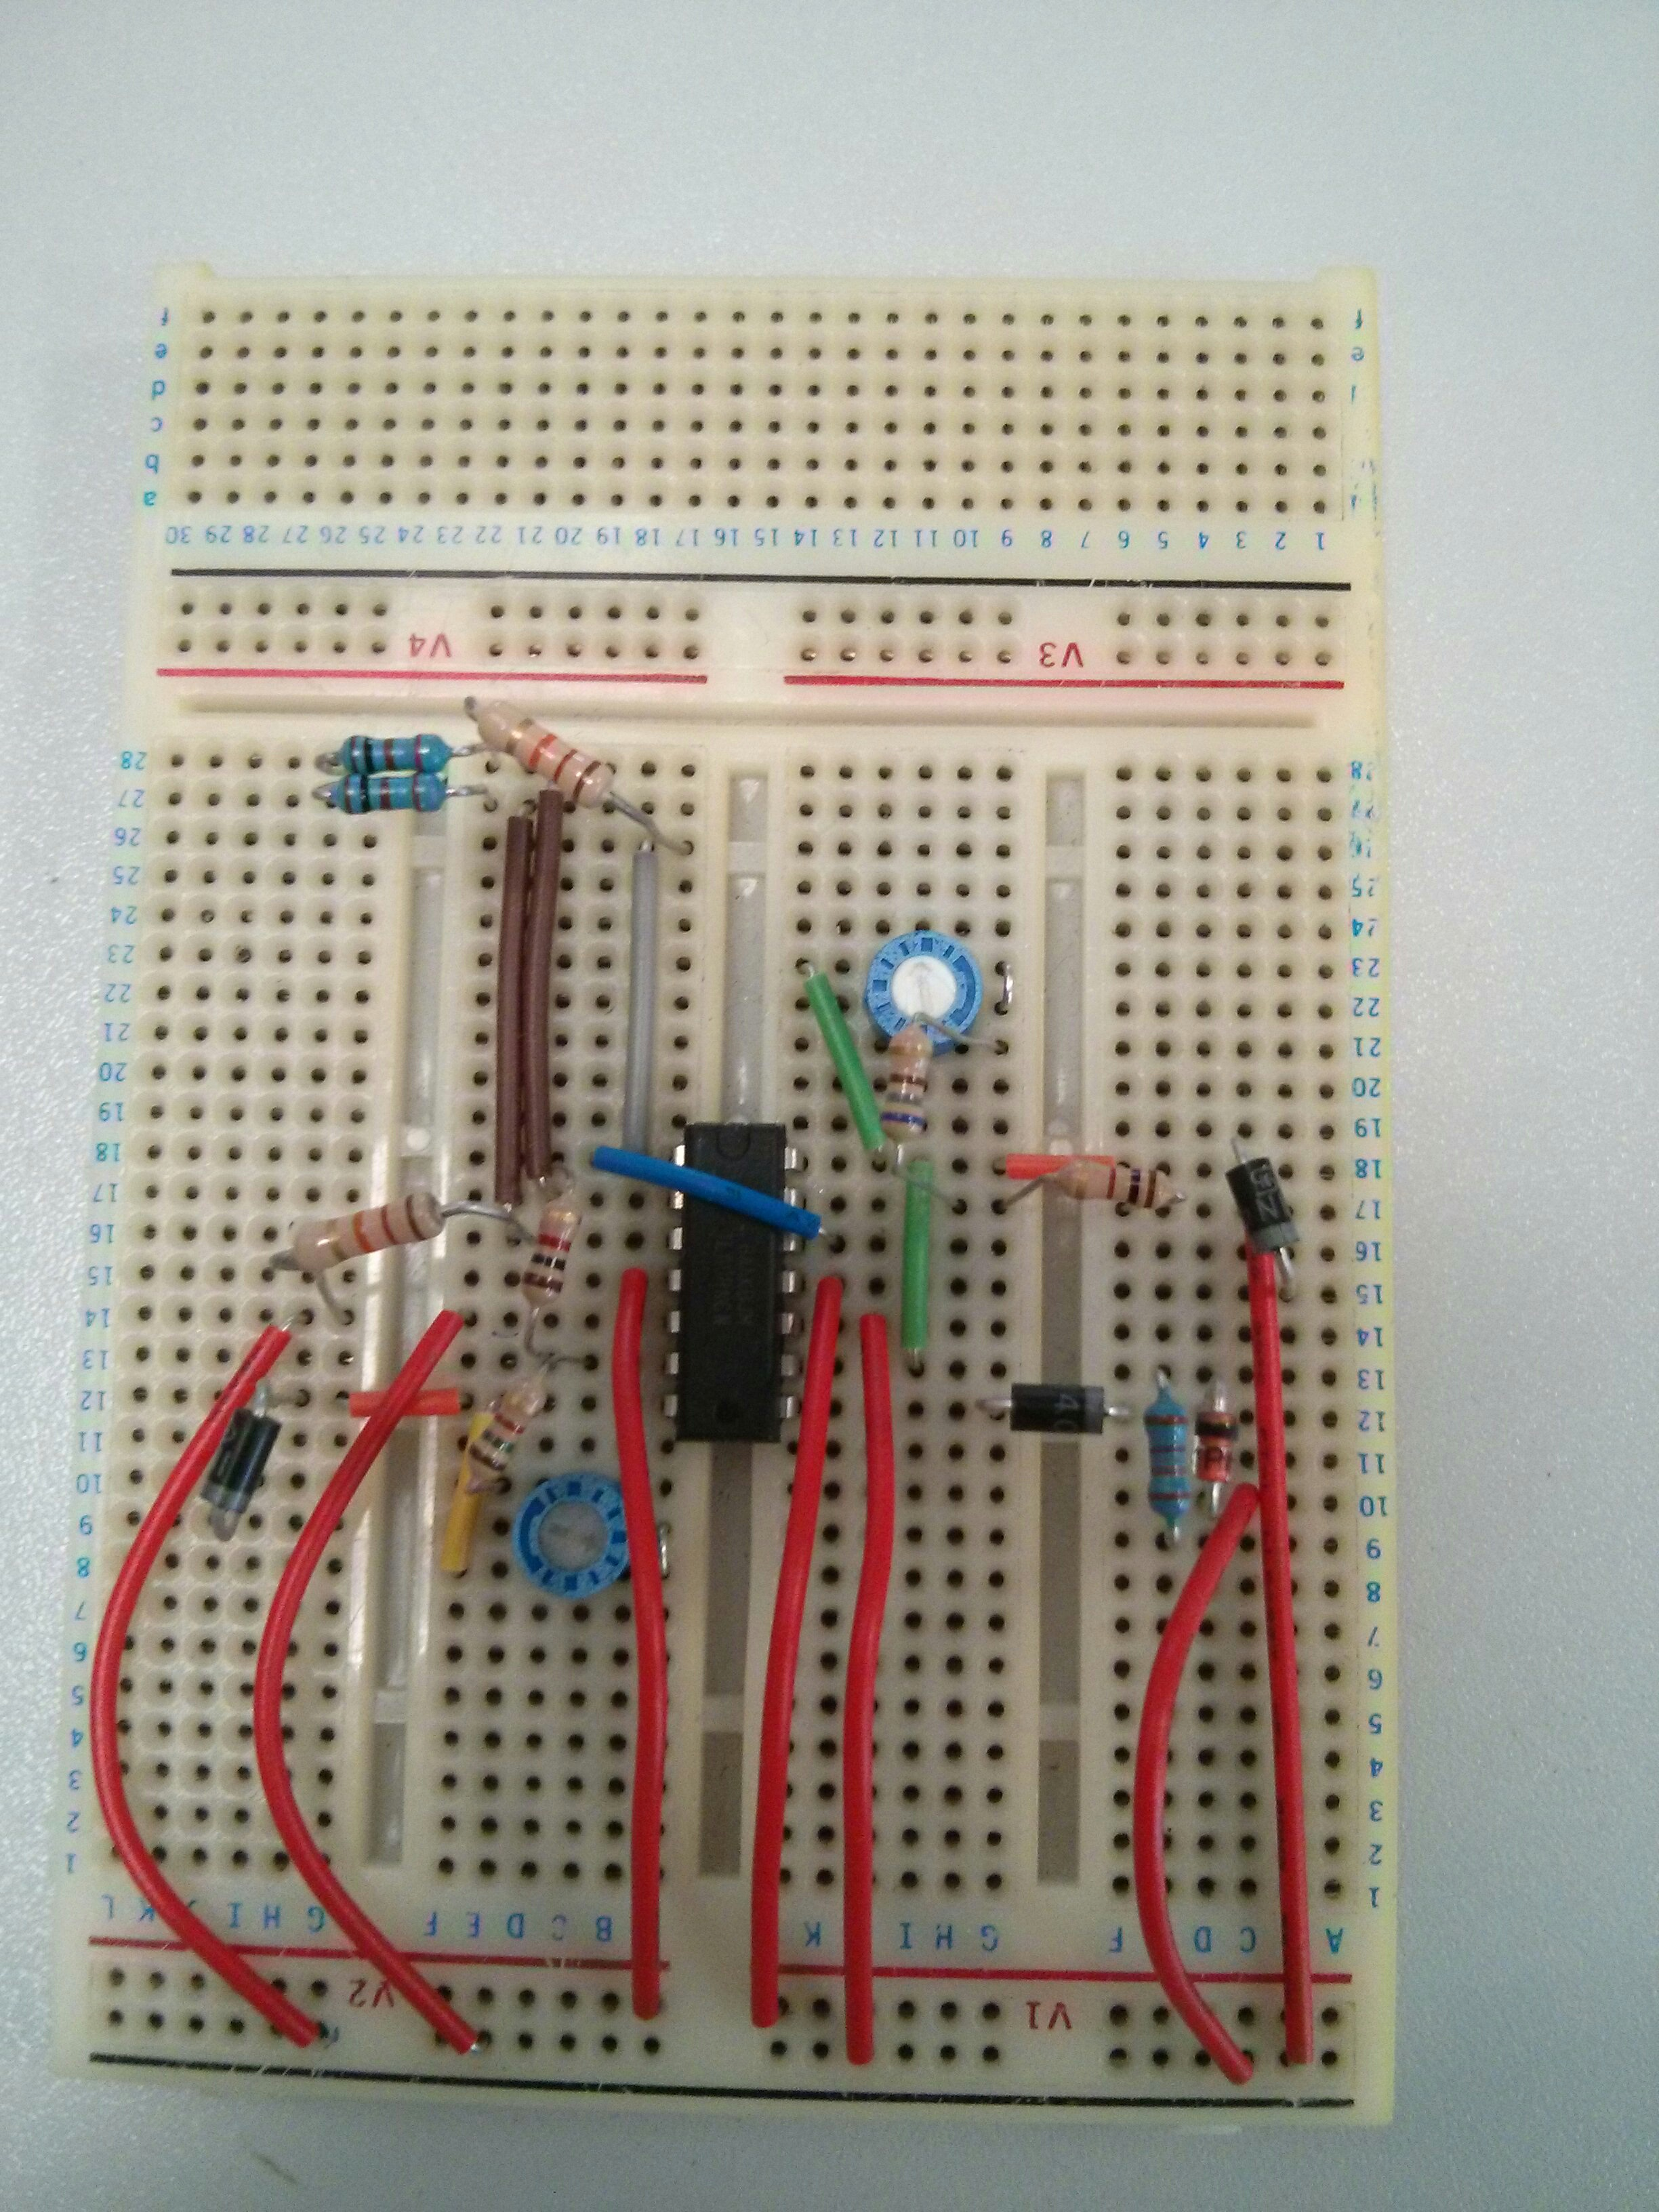
\includegraphics[width=200px]{IMG_20160629_203932.jpg}
    \caption{Montage sur breadboard}
\end{figure}
\FloatBarrier

%%%%%%%%%%%%%%%%%%%%%%%%%%%%%%%%%%%%%%%%%%%%%%%%%%%%%%%%%%%%%%%

\section{Montage Banc d'essai}

Lorsque j'ai pris le projet, la mécanique du banc d'essai n'était pas complète. La conception du banc était terminé, alors que la réalisation du banc était en cours. Certaine pièces était en cours de réalisation par M. Weil. Et d'autre pas encore lancée en fabrication. Aucun câblage électrique réaliser, ni même prévu.

\subsection{Partie Mécanique}

\paragraph{Emplacement du capteur de force \\}

Pour réaliser la mesure de couple, un capteur de force placé avec un bras de levier. La fixation du capteur était prévu avec une plaque fixé en flexion elle même fixer sur le châssis. La décision à été prise de rehausser le châssis et de fixer le capteur directement sur le châssis (par l'intermédiaire d'une plaque d'adaptation. Ce qui permette de concentrer les efforts directement dans le châssis, qui peut être considérer infiniment rigide par rapport aux efforts maximum ($+/- 500 N$).\\
\\
Une fois la décision prise pour le nouvelle emplacement du capteur de force, l'ensemble du châssis fût finaliser. Les montages mécanique du châssis à été donc terminé.

\begin{figure}[!h]
    \centering
    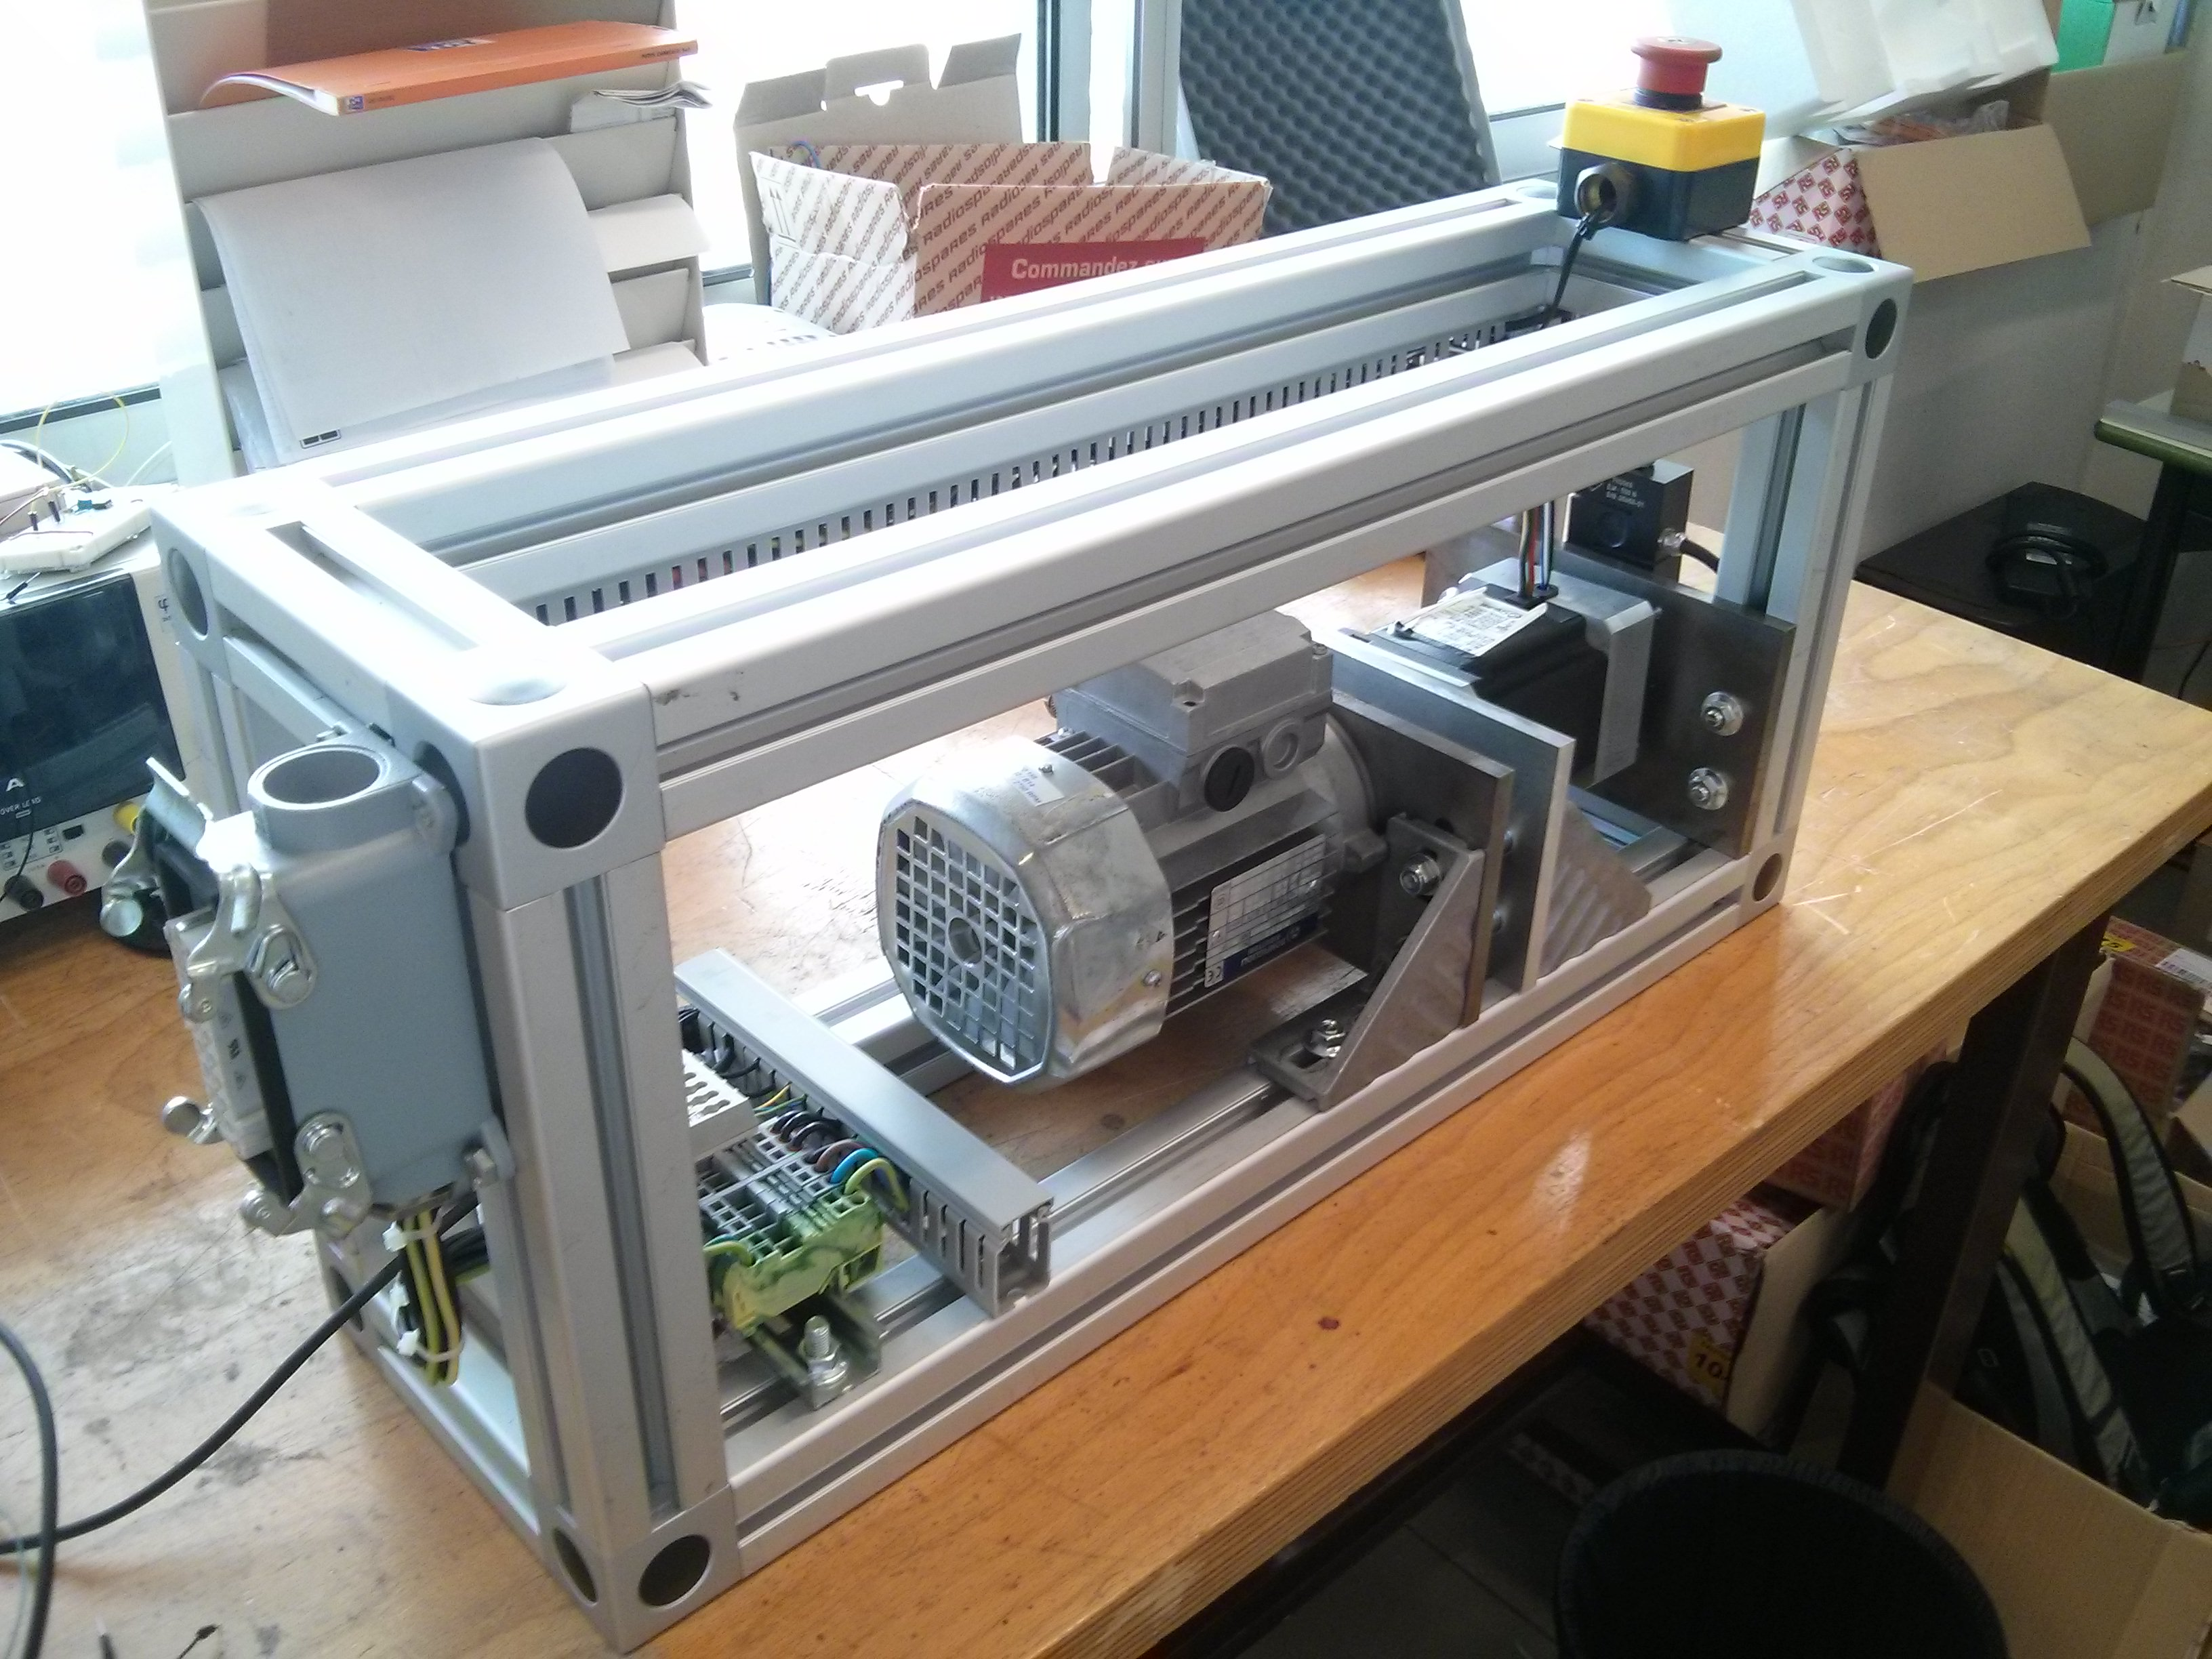
\includegraphics[width=350px]{IMG_20160628_183024.jpg}
    \caption{Banc complet}
\end{figure}

\subsection{Partie électrique}

\subsubsection{Banc d'essai}

Pour une facilité de déplacement et pour permettre de dissocier l'armoire du banc, une prise pour la partie puissance à été mise, cependant pour l'instant il n'y a pas de prise pour la partie logique. Des goulottes et des borniers sont placé pour plus de propreté. Seule le capteur de force ne passe par par le bornier générale du banc, sont câble est suffisamment long mais aussi pour minimiser des problème d'interférence sur la mesure de force.


\begin{figure}[!h]
    \centering
    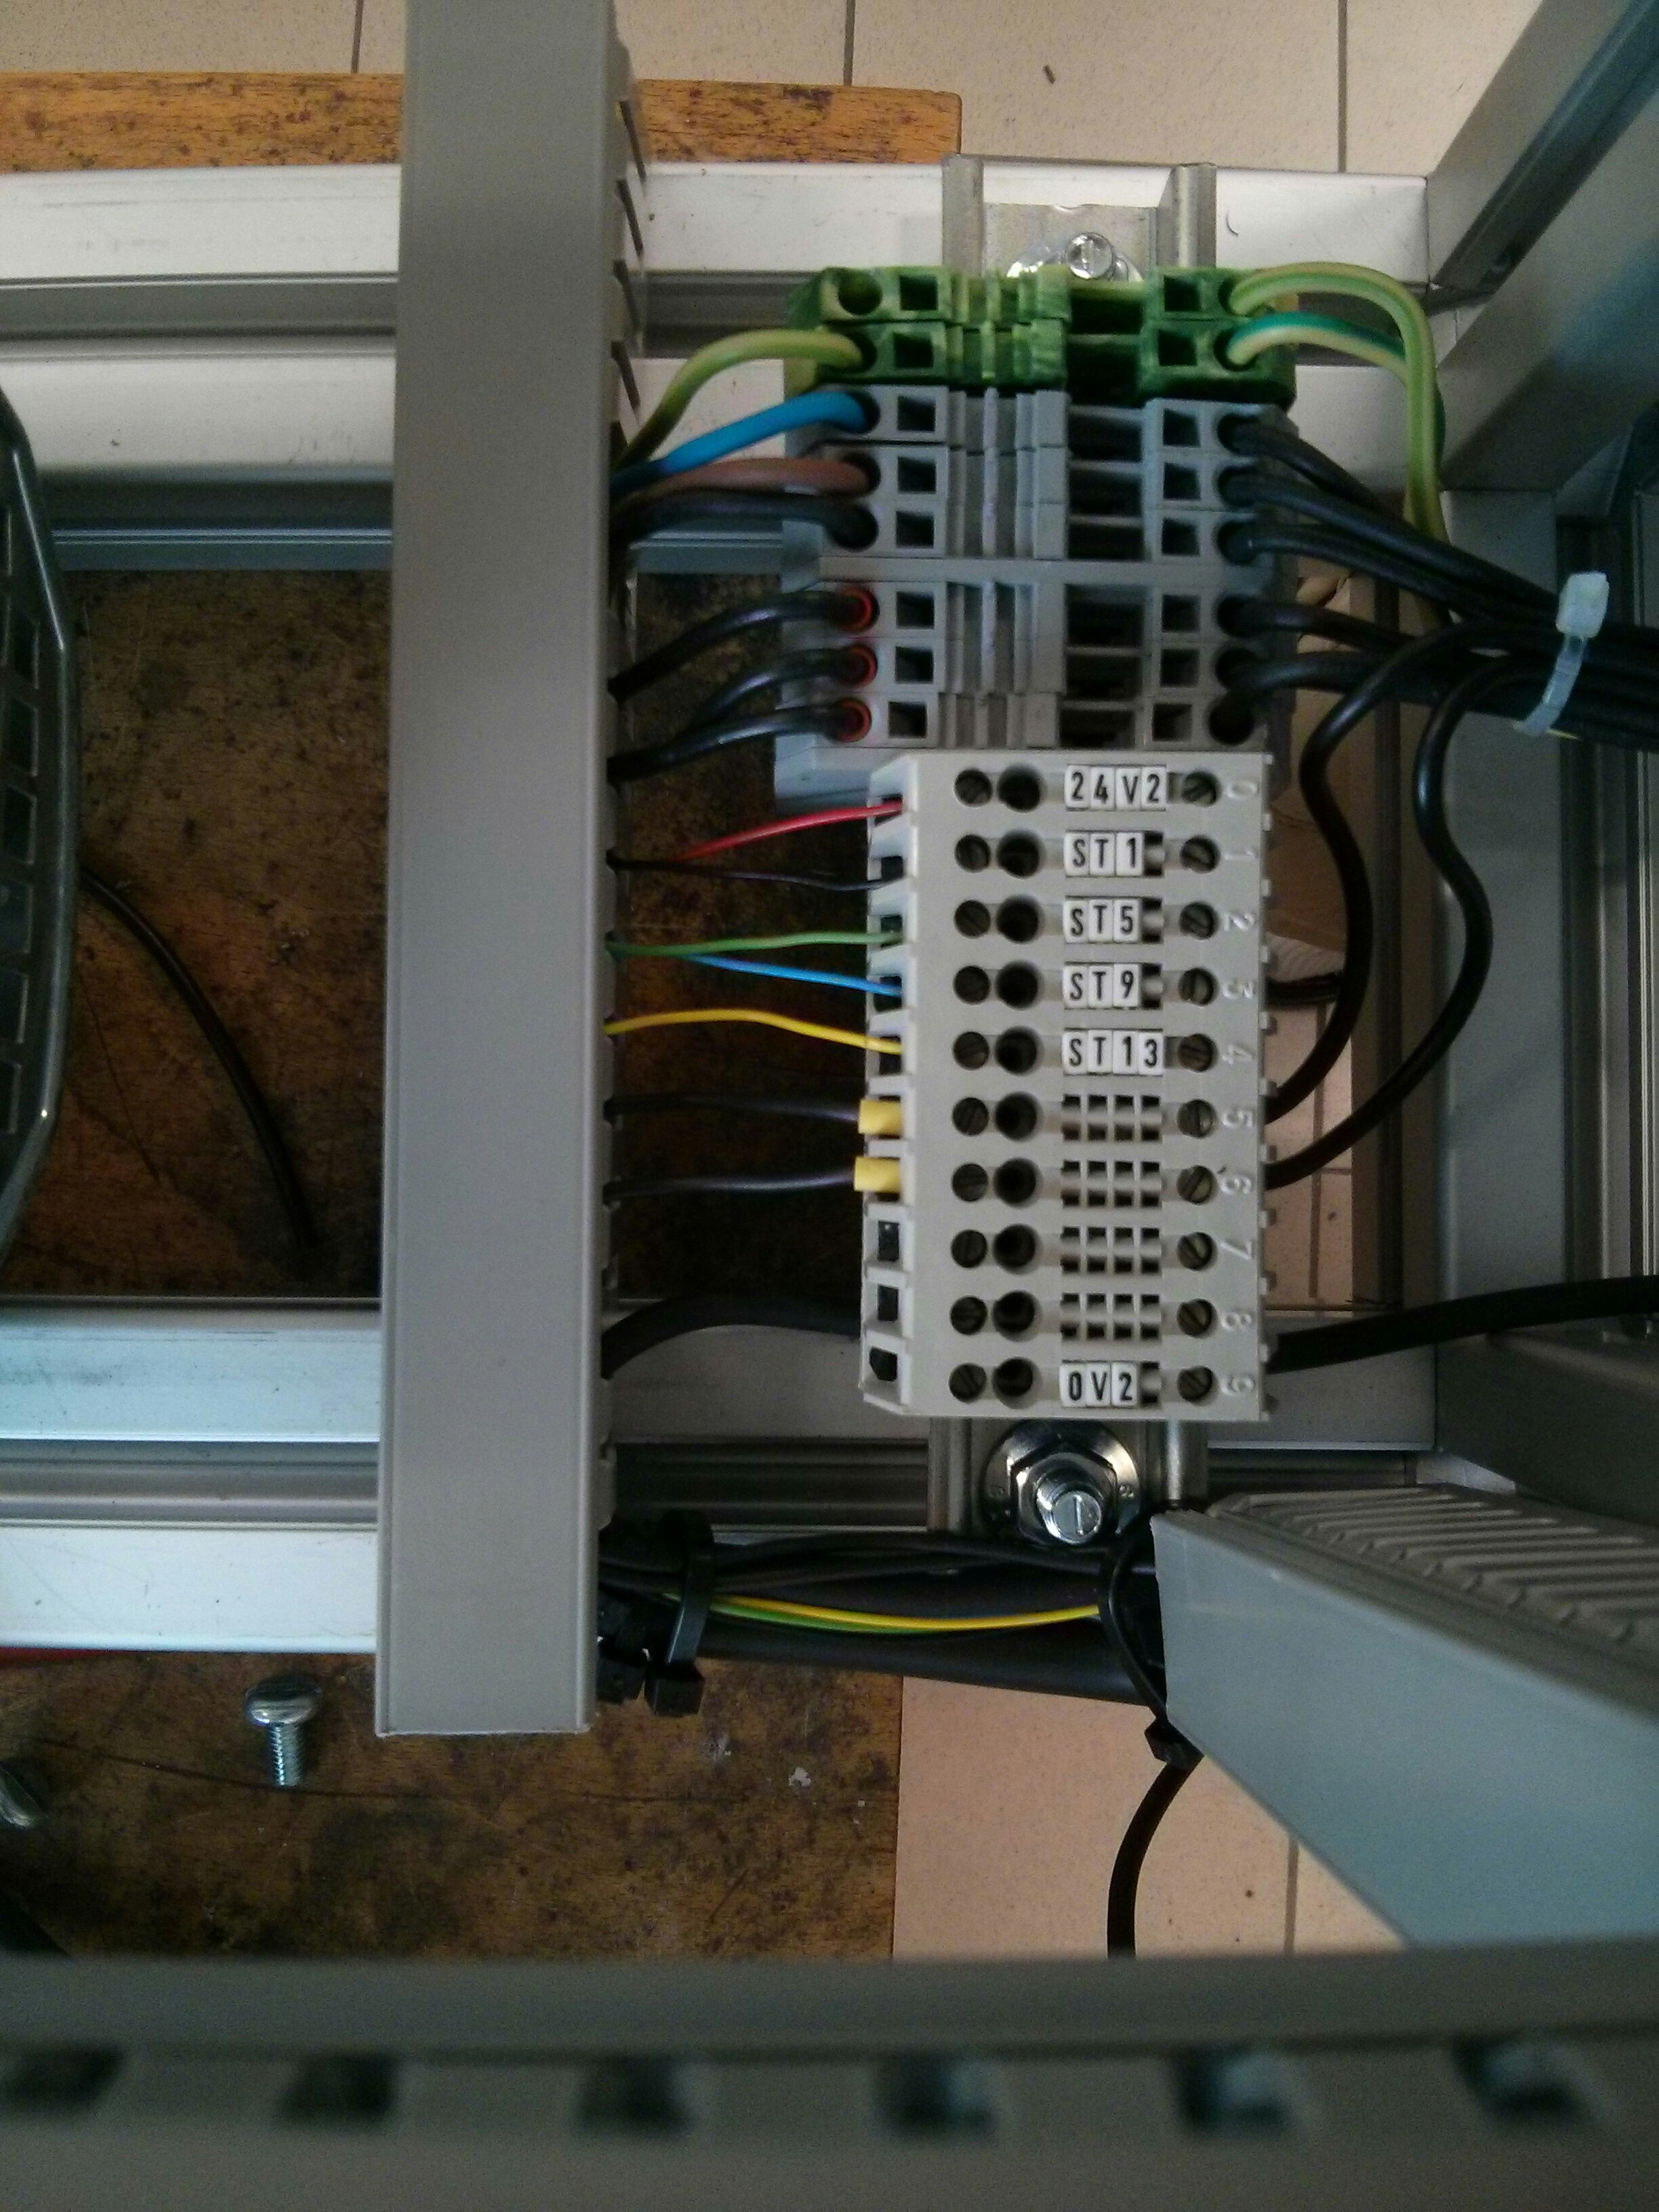
\includegraphics[width=250px]{IMG_20160628_173723.jpg}
    \caption{Bornier du banc d'essai}
\end{figure}


\begin{figure}[!h]
    \centering
    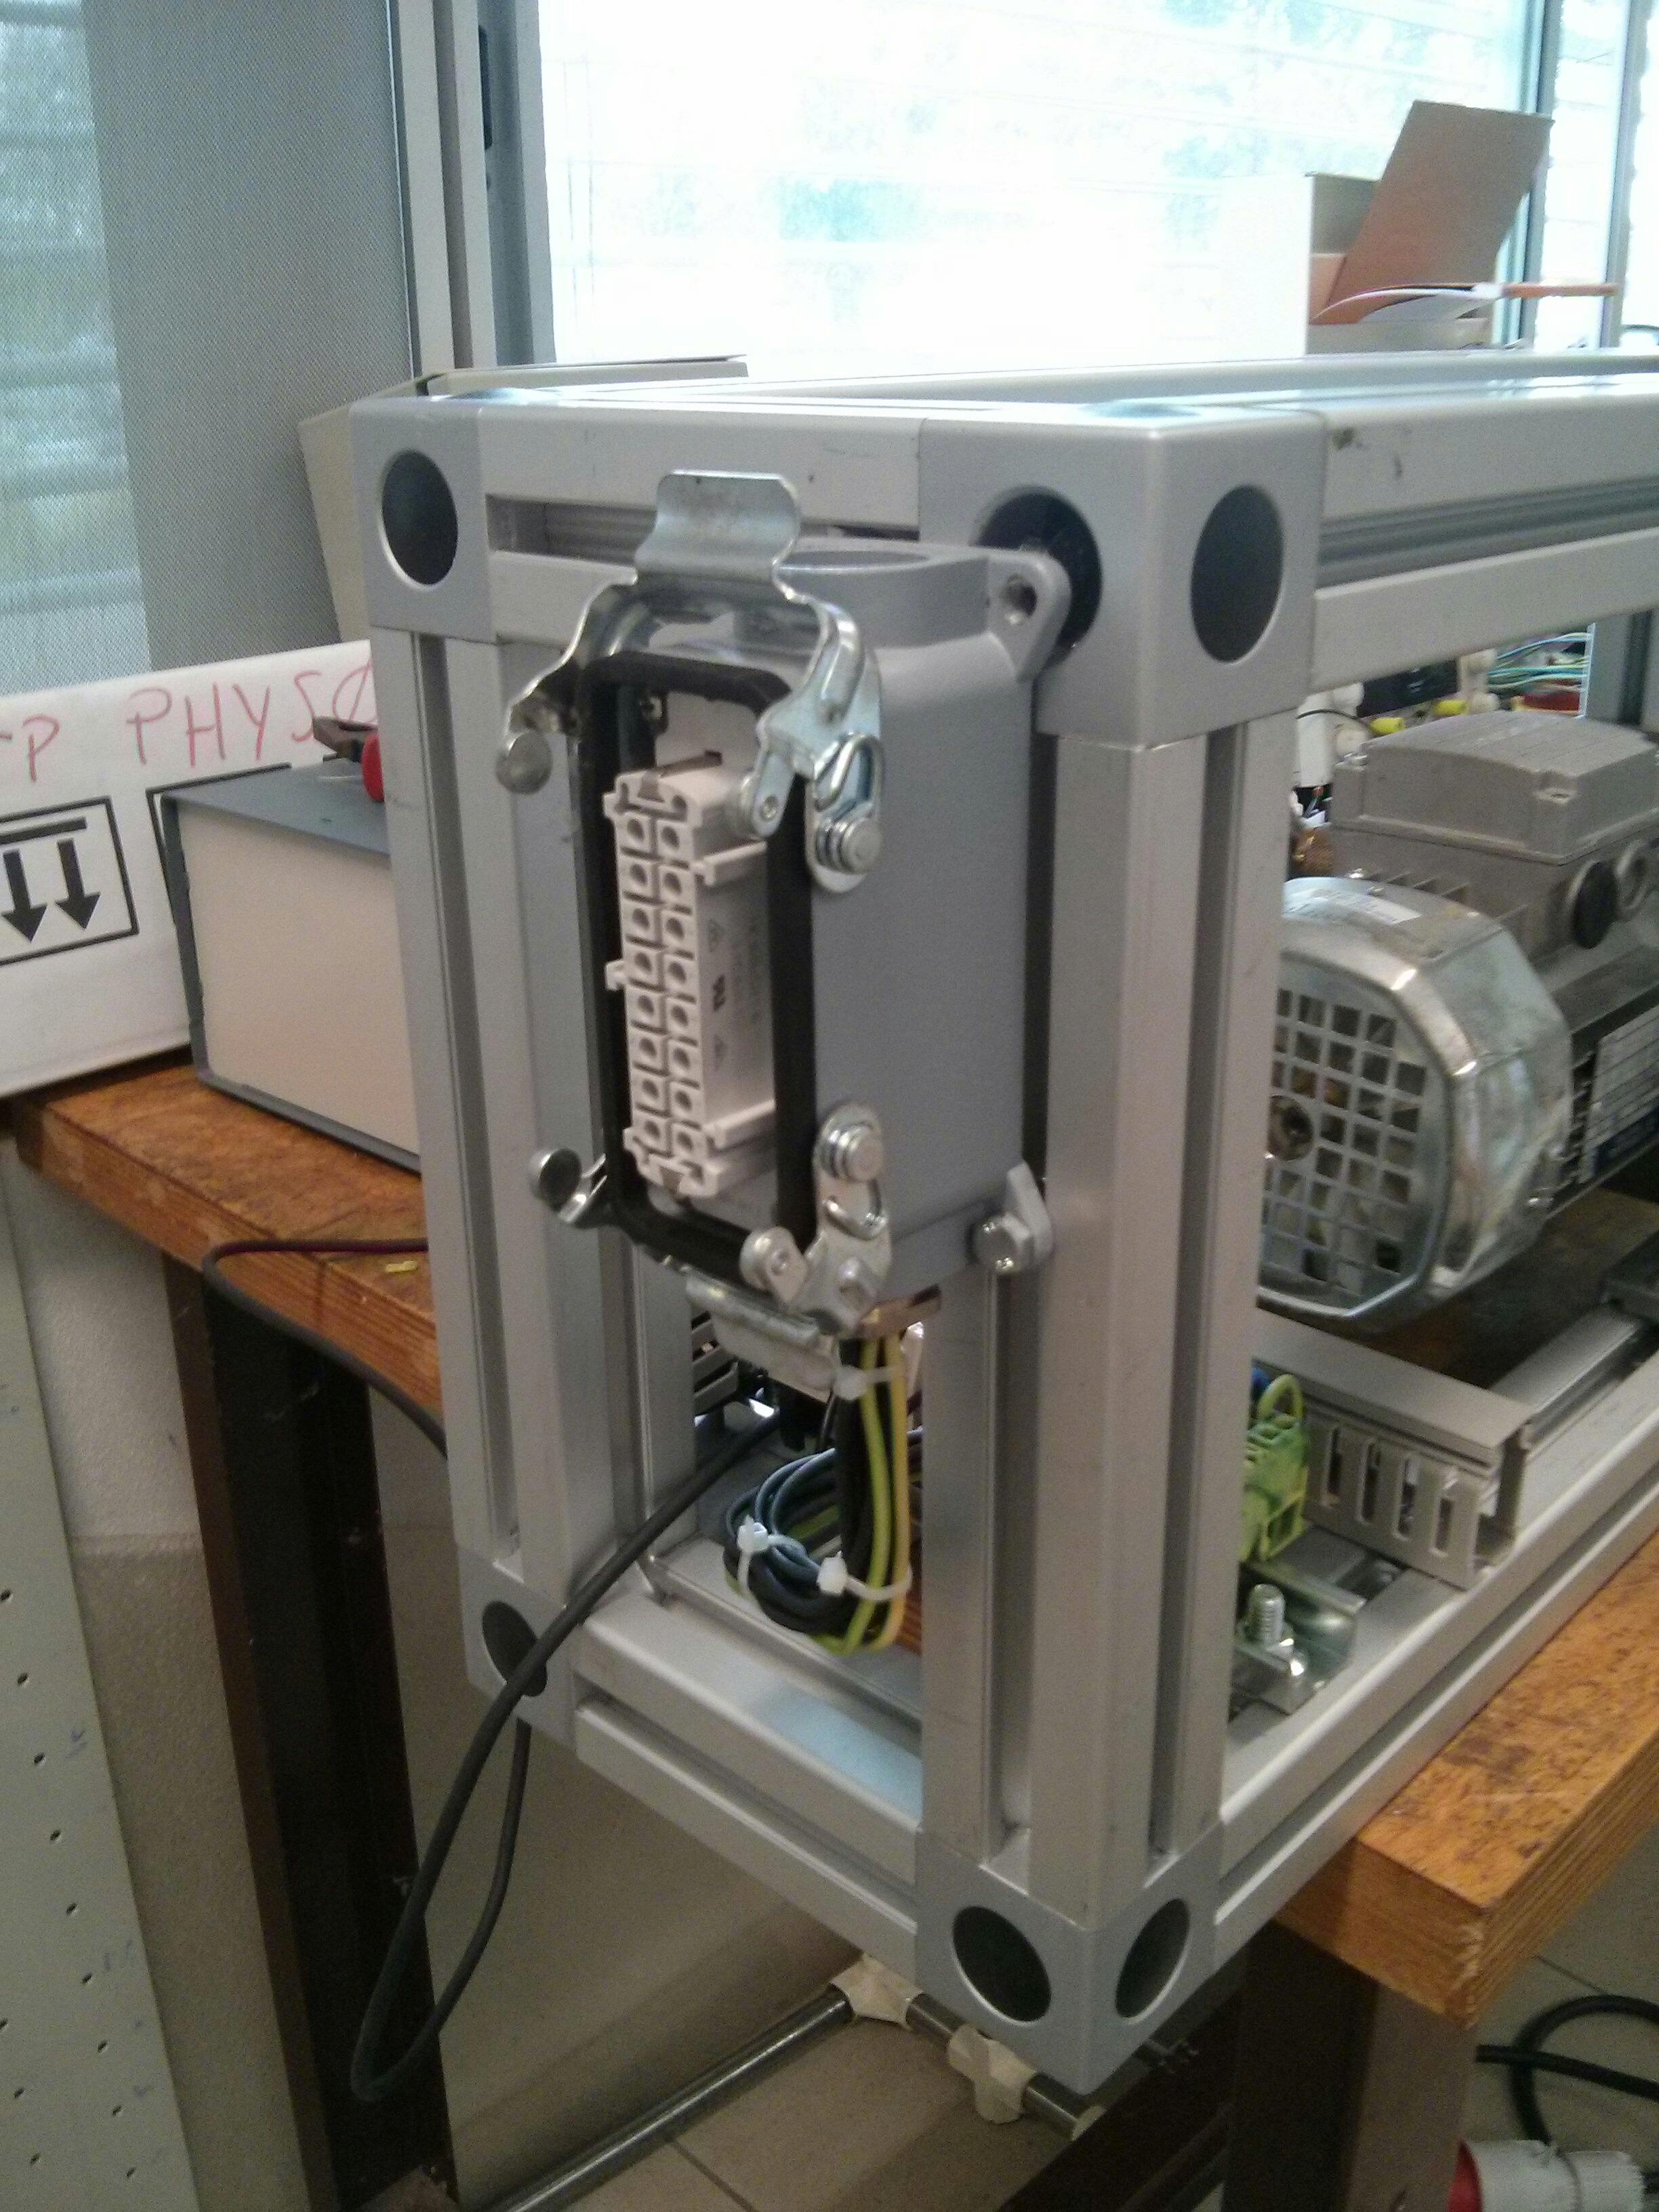
\includegraphics[width=250px]{IMG_20160628_173711.jpg}
    \caption{Prise de puissance pour le banc d'essai}
\end{figure}

\FloatBarrier

\subsubsection{Armoire électrique}
La réalisation de l'armoire est donc basé sur des armoire déjà fabriqué pour d'autre banc d'essai. Mon armoire comporte en plus la partie sur le Brushless.\\
\\
J'ai apporter quelque modification et ajout :

\paragraph{Modification \\}

Passage de l'ensemble de la puissance en tétra, pour le besoin du contrôleur Brushless
	\begin{itemize}
		\item Sectionneur tétra
		\item Disjoncteur 10A tétra
		\item Relais tétra (il devait y avoir une relais tétra, mais pour l'instant il y a un relais tri)
	\end{itemize}

\paragraph{Ajouts\\}

La partie de commande du Brushless est placé dans l'armoire mais aussi l'alimentation de la partie logique.

\begin{itemize}
	\item Contrôleur Brushless avec son alimentation 24V DC 240W
	\item Alimentation de la partie logique par un transformateur 12VDC
\end{itemize}

L'ensemble des éléments sont placé dans l'armoire ,un maximum de rail DIN est placé pour pourvoir rajouté des éléments au besoin. Les goulottes sont placé entre tous les rail DIN, puis l'ensemble est câblé. 

\begin{figure}[!h]
    \centering
    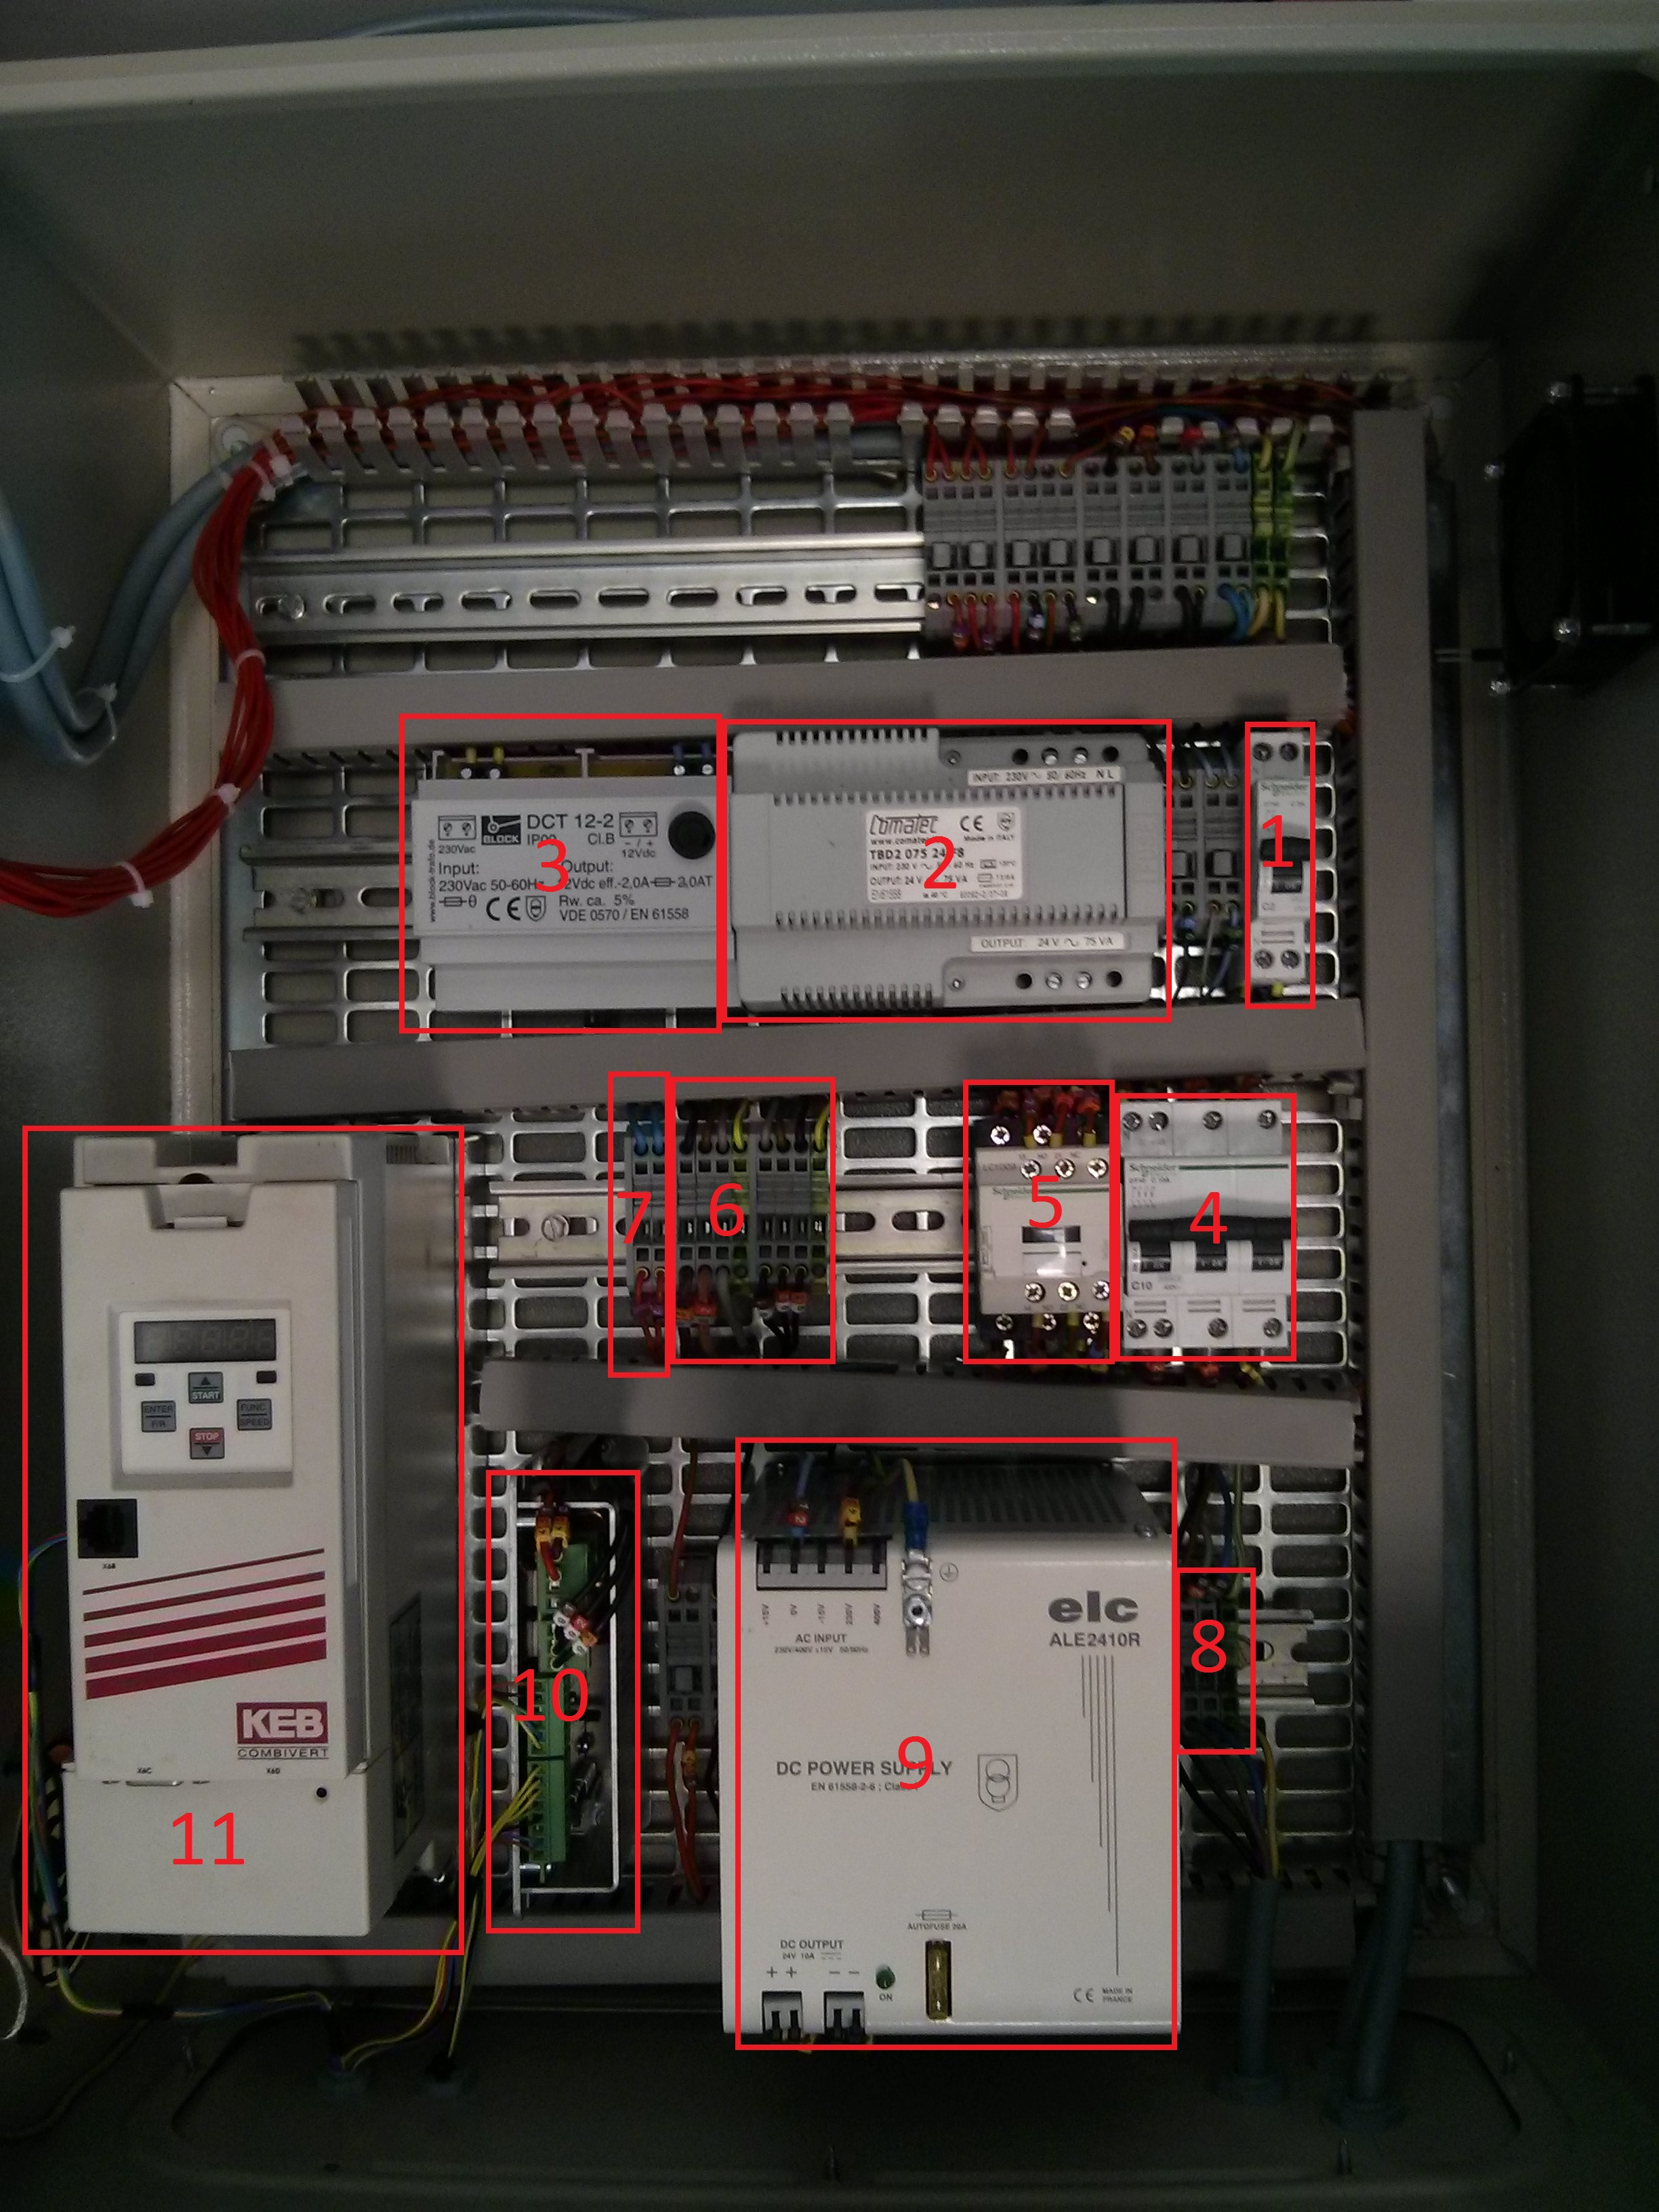
\includegraphics[width=450px]{IMG_20160629_193634.jpg}
    \caption{Intérieur de l'armoire}
\end{figure}
\FloatBarrier
\begin{enumerate}
	\item Protection 2A logique
	\item Transformateur 24V alternatif
	\item Transformateur 12VDC
	\item Protection 10A tétra puissance
	\item Relais tri
	\item Branchement moteur Brushless et moteur asynchrones
	\item Raccordement arrêt d'urgence banc d'essai
	\item Raccordement EDF
	\item Transformateur 24VDC 240W, alimentation brushless
	\item Contrôleur brushless
	\item Variateur asynchrone
\end{enumerate}
%%%%%%%%%%%%%%%%%%%%%%%%%%%%%%%%%%%%%%%%%%%%%%%%%%%

\section{Amélioration futur}

Le banc est fonctionelle mais pas encore complètement fini. Il reste quelque élement à finir.

\begin{itemize}
	\item Cartériser le banc
	\item Faire un support pour l'armoire électrique
	\item Faire une carte électronique complète
\end{itemize}

La partie éléctronique devait être alimenter par le biais de l'armoire éléctrique, il manque pour l'instant un régulateur $10VDC$, et un régulateur $+/- 12VDC$.
%%%%%%%%%%%%%%%%%%%%%%%%%%%%%%%%%%%%%%%%%%%%%%%%%%%

\newpage
\section{Conclusion}

Le projet est pleinement opérationnelle, et permet au prochain semestre la mise en place de TP pour E03, et pour les semestre d'après les TP EA01 et EQ04. Il reste certe quelque élements pour finir le banc mais il est pour l'instant utilisable.


\newpage
%%%%%%%%%%%%%%%%%%%%%%%%%%%%%%%%%%%%%%%%%%%%%%%%%%%
\section{Annexe}

\subsection{Annexe I : Commande Brushless}

\begin{figure}[!h]
    \centering
    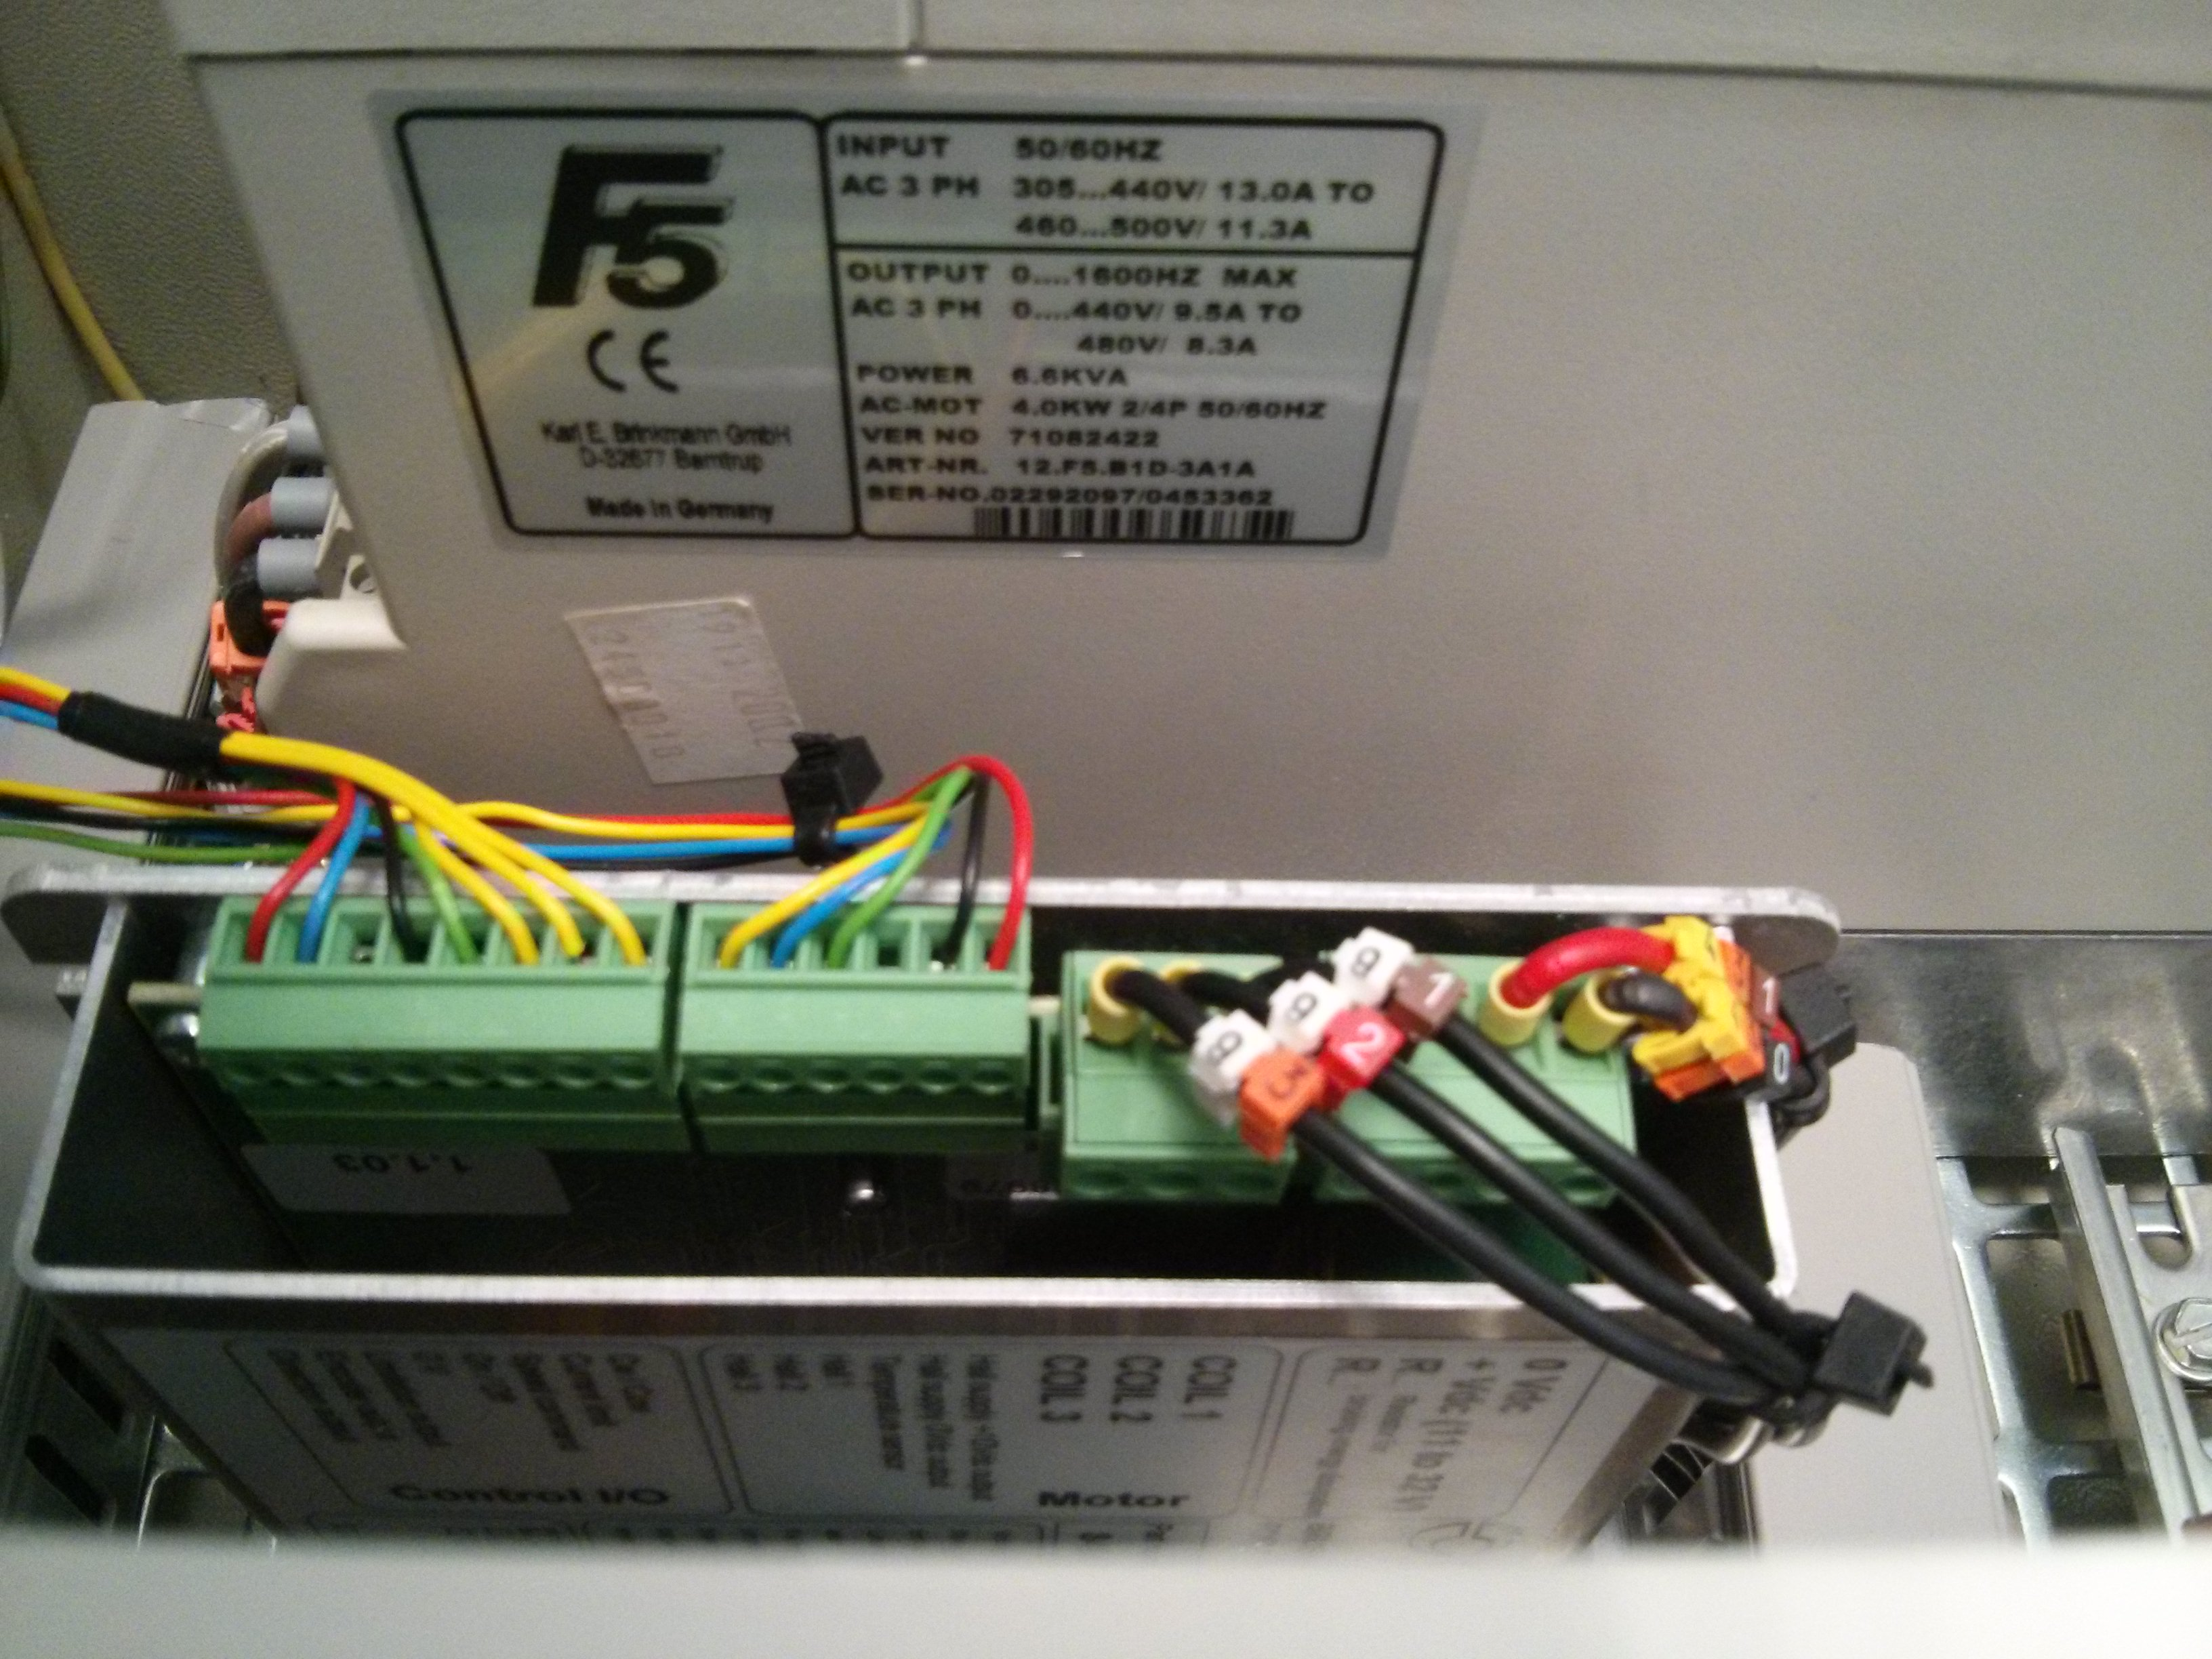
\includegraphics[width=350px]{IMG_20160629_193653.jpg}
    \caption{Câblage contrôleur Brushless}
\end{figure}

\paragraph{Alimentation contrôleur}
\begin{itemize}
	\item GND
	\item +24VDC
	\item Résistance de dissipation (Non-connecté)
	\item Résistance de dissipation (Non-connecté)
\end{itemize}

\paragraph{Alimentation moteur}

\begin{itemize}
	\item Phase 1
	\item Phase 2
	\item Phase 3
\end{itemize}

\paragraph{Capteur moteur}

\begin{itemize}
	\item +VDC (Rouge)
	\item GND (Noir)
	\item Température (Non-connecté)
	\item Effet Hall 1 (Vert)
	\item Effet Hall 2 (Bleu)
	\item Effet Hall 3 (Jaune)
\end{itemize}

\paragraph{Contrôle\\}

\textbf{Input} 

\begin{itemize}
	\item Sens de rotation (Jaune) Commande digital
	\item Limite de courant (Jaune) Commande analogique 0-10VDC
	\item Commande de vitesse (Jaune) Commande analogique 0-10VDC
	\item Marche/Arrêt (Vert) Commande Digital
	\item GND
\end{itemize}

\textbf{Output}

\begin{itemize}
	\item Sortie limitation de courant (Non-connecté)
	\item Sortie encodeur (Bleu) Digital
	\item Sens de rotation réel (Rouge) Digital
\end{itemize}

\newpage

\subsection{Annexe II : Commande Asynchrone}

\begin{figure}[!h]
    \centering
    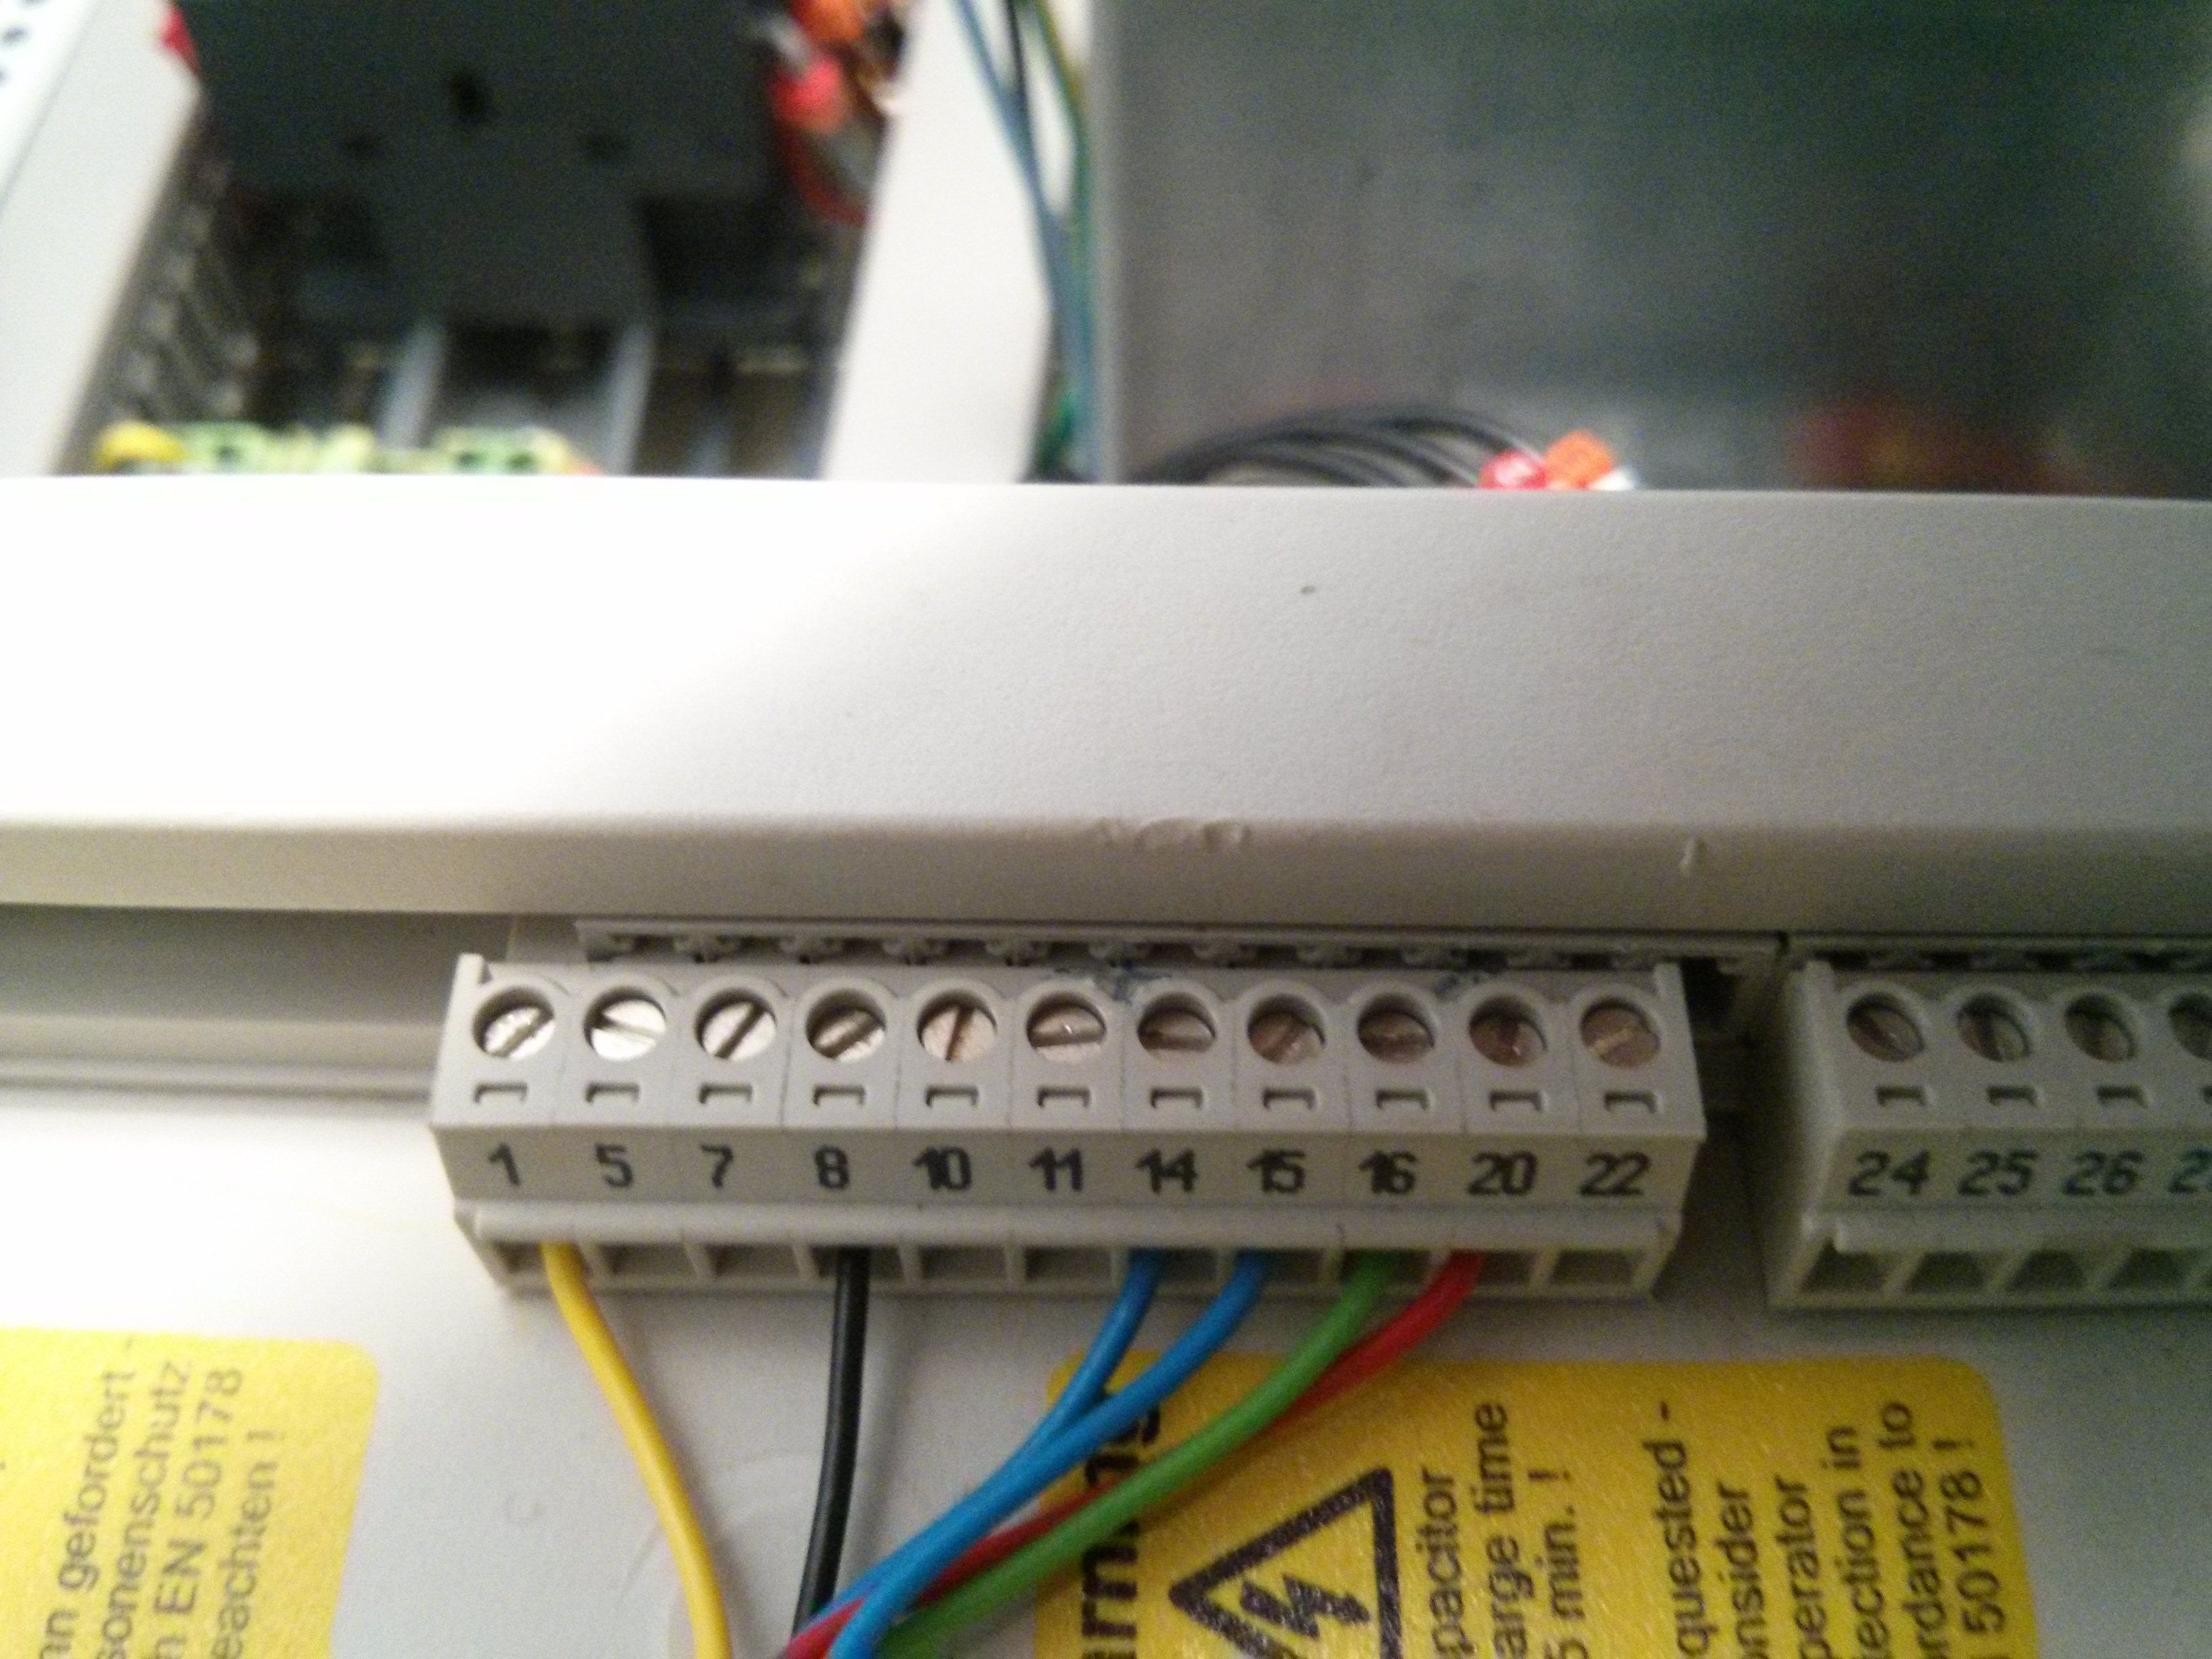
\includegraphics[width=350px]{IMG_20160629_193715.jpg}
    \caption{Branchement de la commande du variateur asynchrone}
\end{figure}

\begin{itemize}
	\item (1) Commande de vitesse (Jaune) Commande analogique 0-10VDC
	\item (8) GND
	\item (14) Forward (Bleu) Commande digital 24VDC
	\item (15) Reverse (Bleu) Commande digital 24VDC (Priorité sur le forward)
	\item (16) Reset (Vert) Commande digital 24VDC
	\item (20) +24VDC
\end{itemize}

\newpage

\subsection{Annexe III : Capteur de force}

\begin{figure}[!h]
    \centering
    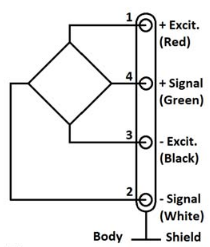
\includegraphics[width=150px]{cablage_fn3060.png}
    \caption{Branchement capteur de force}
\end{figure}

\begin{itemize}
	\item +10VDC  Rouge
	\item +Signal Vert
	\item GND     Noir
	\item -Signal Blanc
\end{itemize}



\end{document}  